\documentclass[journal,10pt]{IEEEtran}
\usepackage{graphicx}
\usepackage{booktabs}
\usepackage{amsmath,amssymb}
\usepackage{array}
\usepackage{cite}
\usepackage{url}
\usepackage{xcolor}
\graphicspath{{figures/}}
\hyphenation{dis-agree-ment inter-po-la-tion re-con-struc-tion}

\begin{document}
\title{Measurement Dependence Governs Disagreement-Based Reliability in Deterministic MRI Slice Interpolation: A Three-Cohort Characterization}
\author{Anonymous Authors% Author names, affiliations, funding, and corresponding author required before submission.
}
\markboth{IEEE Transactions on Medical Imaging, Manuscript Under Preparation}{}
\maketitle

\begin{abstract}
Deterministic through-plane MRI interpolation can produce plausible missing slices without indicating when they are inaccurate. Disagreement between reconstructions is a natural reliability signal, but it observes only differences between their errors and can miss common-mode failures. We characterize the hypothesis that shared acquired slices control this blindness. Two frozen neural interpolators reconstructed identical missing physical planes under measurement-disjoint and maximal-shared $\times4$ contexts. The study covers 24 fastMRI brain T2 examinations, 115 IXI brain T2 examinations, and 22 NingXia knee T2 series from eight patients. Dense targets were used only to synthesize retrospective acquisitions and evaluate error. Across two architectures and seven endpoints, all 42 disjoint-minus-shared ranking differences were positive; MAE differences were 0.077--0.132 on fastMRI/IXI and 0.107--0.147 on NingXia. Shared error fraction was strongly associated with suppressed normalized disagreement after controlling total error and examination (partial Spearman $-0.746$ to $-0.975$). Analytical interpolation independently showed that, from $\times2$ to $\times6$, shared fraction rose monotonically while disagreement--error ranking fell in every cohort. Geometry was exact for 322 outputs; common-scale normalization preserved the directional contrast, whereas independent output normalization was invalid. Measurement-disjoint scores achieved nAURC 0.0119/0.0013/0.0107 on fastMRI/IXI/NingXia, outperforming shared-anchor and committee disagreement, but an adjacent-anchor baseline was stronger on NingXia. Stable-wrong events were coherent but rare. The supported principle is scoped: reliability contexts should reduce shared error-generating measurements rather than merely maximize output diversity. Low disagreement cannot certify correctness, and the study does not establish calibrated uncertainty or clinical safety.
\end{abstract}

\begin{IEEEkeywords}
Magnetic resonance imaging, slice interpolation, image reconstruction, reliability, uncertainty estimation, consistency, sampling.
\end{IEEEkeywords}

\section{Introduction}
\IEEEPARstart{A}{nisotropic} magnetic resonance imaging (MRI) volumes often have substantially coarser through-plane than in-plane resolution. Interpolating unacquired slices can ease visualization and downstream volumetric processing, and modern slice-synthesis networks improve over classical interpolation in many settings \cite{peng2020saint,song2024i3net}. Yet a deterministic interpolator normally returns one image, even when the acquired anchors do not constrain the missing anatomy sufficiently. A deployment-facing reliability signal must therefore identify likely failure without accessing the dense target that is missing in practice.

Model ensembles, stochastic sampling, test-time augmentation (TTA), and cross-context consistency estimate reliability from variation among plausible outputs \cite{gal2016dropout,lakshminarayanan2017ensembles,edupuganti2021uncertainty,narnhofer2022bayesian}. Their common premise is useful but one-sided: disagreement witnesses that at least one prediction differs, whereas agreement need not imply correctness. If two reconstructions inherit the same smoothing, boundary limitation, or anchor-induced bias, subtracting them removes the very error one wishes to detect. This issue is especially relevant to interpolation because nearby reconstruction contexts can reuse the same acquired slices.

We investigate measurement overlap as a control variable for error observability (Fig.~\ref{fig:concept}). The same missing physical plane is reconstructed twice at the same nominal factor. In one condition, the two contexts draw from phase-shifted $\times4$ anchor lattices with no shared slices. In the maximal-overlap control, they use the identical anchor lattice but reverse its through-plane order before mapping the output back. Case, target, model, plane, evaluation support, and number of measurements remain paired. The control has a known limitation---reversal changes ordering---so we interpret it as a mechanistic retrospective intervention, not a complete causal identification of overlap alone.

The study makes five contributions. First, it separates elementary correlated-error algebra from a physically auditable source of error dependence: reuse of acquired slice anchors. Second, it conducts target-preserving measurement-overlap experiments across three cohorts, two anatomies, two neural architectures, and seven endpoints, with patient-level inference for the multi-series knee cohort. Third, it measures consensus-error distributions, stable-wrong prevalence, geometry, and intensity operating ranges rather than relying on a single correlation. Fourth, it evaluates analytical $\times2/\times4/\times6$ factor trends and complete examination-level risk--coverage curves. Fifth, it distinguishes the supported output-based mechanism from a strong acquired-anchor baseline and a retrospective densification consequence. All claims concern deterministic MRI slice interpolation; we do not claim calibrated uncertainty, prospective acquisition benefit, or clinical safety. The contribution is a reliability-design study rather than a new reconstruction backbone: it asks which measurements must change before consistency can carry useful evidence about error.

\begin{figure}[t]
\centering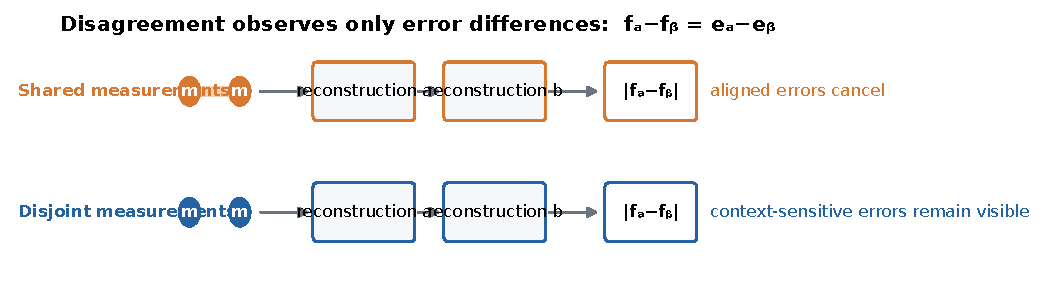
\includegraphics[width=\columnwidth]{fig1_concept.pdf}
\caption{Consensus blindness. When contexts reuse error-generating measurements, aligned errors cancel in output disagreement. Disjoint contexts can reveal a larger context-sensitive component, but agreement still cannot certify correctness.}
\label{fig:concept}
\end{figure}

\section{Related Work}
\subsection{MRI Slice Synthesis and Interpolation}
Classical linear and cubic splines estimate missing samples from smoothness assumptions \cite{deboor1978splines}. Deep slice-synthesis methods instead learn anatomical priors. SAINT conditions synthesis on spatial position and supports variable upsampling factors \cite{peng2020saint}; I3Net combines inter- and intra-slice information for medical slice synthesis \cite{song2024i3net}. These approaches primarily optimize reconstruction fidelity. Our question is complementary: given a frozen deterministic interpolator, which target-preserving contexts expose its retrospective error?

\subsection{Reconstruction Uncertainty and Reliability}
MRI reconstruction uncertainty has been estimated through variational latent models, SURE, Bayesian parameter distributions, and posterior sampling \cite{edupuganti2021uncertainty,narnhofer2022bayesian}. In neuroimage enhancement, predictive uncertainty has also been evaluated against errors and distribution shift \cite{tanno2021uncertainty}. Deep ensembles have been evaluated explicitly under MRI domain shifts \cite{kuestner2024ensembles}. Hu \emph{et al.} showed that variability-based uncertainty can fail to capture systematic reconstruction error \cite{hu2021predict}; consensus blindness itself is therefore not claimed as a new observation. We do not estimate a calibrated posterior. Our narrower question is whether a physical, recorded dependence---reuse of the same acquired slices---changes how much deterministic error is visible in output disagreement.

\subsection{Consistency, Diversity, and Shared Error}
Deep ensembles and stochastic perturbations use diversity as evidence of uncertainty \cite{lakshminarayanan2017ensembles,gal2016dropout}. Ensemble theory emphasizes that diversity interacts with, rather than replaces, individual predictor accuracy \cite{brown2005diversity,ortega2022diversity}. Self-consistency also has a long history in MRI reconstruction, including measurement consistency in SPIRiT \cite{lustig2010spirit}. Leave-one-slice-out evaluation was previously used to compare medical interpolation algorithms \cite{horvath2017highorder}; the held-out operation is therefore not new. Our distinction is intervention-level: we manipulate overlap of acquired through-plane measurements for the same target and quantify error observability and risk ranking, rather than interpreting arbitrary output dispersion as uncertainty.

\section{Theory: Consensus Error and Disagreement Blindness}
Let $y$ be a missing target slice and let two deterministic contexts produce
\begin{equation}
 f_a=y+e_a,\qquad f_b=y+e_b.
\end{equation}
Their difference contains no target term:
\begin{equation}
 f_a-f_b=e_a-e_b,
\end{equation}
and squared disagreement satisfies
\begin{equation}
 \|e_a-e_b\|^2=\|e_a\|^2+\|e_b\|^2-2\langle e_a,e_b\rangle. \label{eq:cov}
\end{equation}
Positive error alignment therefore reduces observable disagreement at fixed marginal error energy. Define the context mean $\bar e=(e_a+e_b)/2$ and half-difference $\delta=(e_a-e_b)/2$. The exact identity
\begin{equation}
 \tfrac12(\|e_a\|^2+\|e_b\|^2)=\|\bar e\|^2+\|\delta\|^2 \label{eq:decomp}
\end{equation}
separates shared consensus error from context-observable diversity. This is an algebraic decomposition, not a calibrated uncertainty partition. It also does not identify which reconstruction is wrong.

An immediate boundary follows from the common-mode case $e_a=e_b=c$. Then $\delta=0$ and disagreement vanishes for every nonzero $c$, while the complete error remains in $\bar e=c$. Conversely, if $e_a=-e_b$, the mean error cancels and all paired energy is observable. Real interpolation contexts lie between these extremes. A reliability intervention is useful only insofar as it rotates or decorrelates relevant error components; changing output appearance without changing their direction relative to the target need not improve observability.

For any metric $d$ obeying the triangle inequality,
\begin{equation}
 d(f_a,f_b)\leq d(f_a,y)+d(f_b,y).
\end{equation}
Thus large disagreement lower-bounds the sum of errors only in a one-sided sense, while small disagreement gives no upper bound. A pair can be stably wrong with $e_a\approx e_b\neq0$. Equation~\eqref{eq:cov} motivates the hypothesis that reducing overlap of error-generating measurements decreases $\langle e_a,e_b\rangle$ and makes error more observable.

\section{Measurement-Overlap Hypothesis}
A \emph{target-preserving context} is a set of acquired anchors and reconstruction operations that predicts the same physical missing plane. Measurement overlap is the number of identical acquired slices shared by the two bracketing contexts. At factor four, phase-0 anchors are $z=0,4,8,\ldots$ and phase-2 anchors are $z=2,6,10,\ldots$. Targets with $z\bmod4\in\{1,3\}$ are missing from both grids, and the two grids share no anchors (Fig.~\ref{fig:design}).

The maximal-overlap control uses the phase-0 anchors in both contexts, reverses the sparse sequence for one run, and maps its prediction back to physical $z$. It shares two bracketing anchors for each interior target. Our prespecified directional prediction is that greater overlap increases error alignment, lowers the observable error fraction, and weakens ranking of target error by disagreement. Plan6 expands the frozen comparison without changing that prediction: it evaluates full energy distributions, seven error endpoints, geometry/intensity perturbations, factors two through six with analytical estimators, and examination-level selective risk. Neural finite-difference influence is reserved for the separate conference mechanism paper and is not used to support the journal conclusions.

\begin{figure}[t]
\centering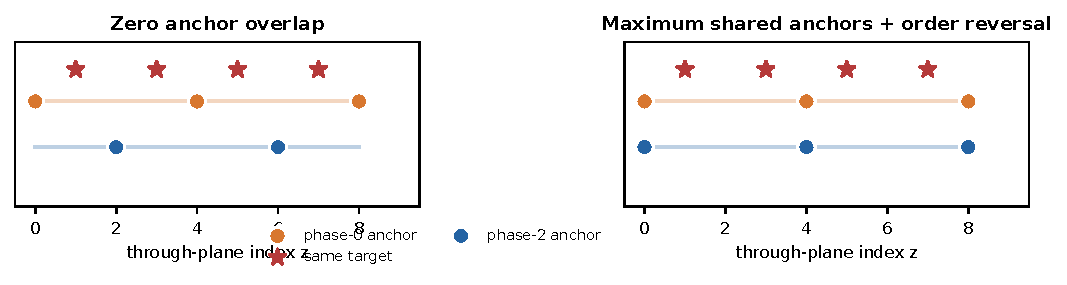
\includegraphics[width=\columnwidth]{fig2_design.pdf}
\caption{Paired $\times4$ design. Stars mark the same evaluated missing targets. The zero-overlap condition changes the phase lattice; the maximal-overlap control reuses the phase-0 anchors under order reversal.}
\label{fig:design}
\end{figure}

\section{Materials and Methods}
\subsection{Data and Units of Analysis}
Table~\ref{tab:data} summarizes the cohorts. The expanded fastMRI-brain-T2 subset contained 160 NIfTI volumes split 112/24/24; all Plan6 analyses used the 24-case test partition. The underlying fastMRI resource is public and deidentified \cite{zbontar2018fastmri,knoll2020fastmri}. IXI-T2 \cite{ixi_dataset} contributed 115 held-out brain MRI examinations and now enters every structurally eligible principal characterization. NingXia-T2 contained 22 knee MRI series from eight patients. Predictions were strictly out of fold under eight patient-group folds; inferential resampling uses the patient prefix rather than treating 22 series as independent. This corrects the historical record without changing stored point estimates.

Inclusion required matching case identity, finite arrays, equal in-plane dimensions, and a valid NIfTI affine. Generated planes were matched in world coordinates by their affine-derived origins within 0.001~mm. Acquired anchors were excluded. No registration or post-validation resampling was allowed.

\begin{table}[t]
\caption{Cohorts and frozen experimental roles}
\label{tab:data}\centering
\begin{tabular}{p{1.05cm}p{.72cm}p{1.25cm}p{.58cm}p{2.3cm}}
\toprule
Cohort & Site & Unit $N$ & $r$ & Role \\
\midrule
fastMRI T2 & brain & 24 cases & 2/4/6 & Neural overlap; analytical factors; risk \\
IXI T2 & brain & 115 cases & 2/4/6 & Neural overlap; analytical factors; risk \\
NingXia T2 & knee & 8 patients / 22 series & 2/4/6 & OOF neural overlap; analytical factors; risk \\
\bottomrule
\end{tabular}
\end{table}

\subsection{Reconstruction Methods}
The controlled neural experiments used frozen 2.5-D HAT and SwinIR interpolators. They process adjacent acquired slices and synthesize the missing interval; checkpoints and standard predictions were fixed before Plan6. No model was refit to optimize a reliability endpoint. For neural multi-endpoint and distribution experiments, three eligible physical planes per examination were selected by a deterministic rule, giving 96 fastMRI, 7,104 IXI, and 124 NingXia model--plane observations per context after all target-preserving positions were aggregated. I3Net remained excluded from the disjoint phase intervention because the frozen implementation required four input slices where several volumes provided only three phase-shifted anchors; we did not pad uncovered outputs.

The factor experiment used two analytical estimators that remain defined in shallow volumes at $\times6$: two-anchor linear interpolation and nearest-anchor replication. This choice deliberately differs from the earlier linear/cubic family check. Four-anchor cubic interpolation was infeasible for a nontrivial fraction of shallow $\times6$ series, and silently retaining only deep volumes would have changed the cohort. Analytical factors are an estimator-family robustness experiment, not a proxy for absent neural outputs.

\subsection{Reliability Scores and Endpoints}
For paired predictions $a,b$, the primary plane score was mean absolute disagreement on the deployment mask $|a|>0.01\max|a|$. Dense targets entered only phase-grid simulation and retrospective evaluation, never the reliability score. The seven endpoints were MAE, RMSE, MSE, $1-\mathrm{SSIM}$, gradient MAE, Gaussian low-frequency MAE, and residual high-frequency MAE. The first three quantify intensity-domain magnitude; the next separates structural similarity; the final three test whether the relation is confined to low-frequency appearance. Examination or model--series scores were medians across matched generated planes.

For paired errors $e_a,e_b$, total energy was $T=(\|e_a\|^2+\|e_b\|^2)/2$, shared energy was $S=\|\bar e\|^2$, observable energy was $O=\|\delta\|^2$, and shared fraction was $q=S/(S+O)$. Error cosine was the centered cosine between $e_a$ and $e_b$. A strict stable-wrong plane had error above the pooled within-dataset/model 75th percentile and disagreement below the 25th percentile. Thresholds were computed once across the two contexts; they were not tuned per condition.

Frozen secondary comparators included: (i) target-excluded committee disagreement; (ii) Physical Consistency (PC-v1), the median absolute difference among NIfTI-affine matched predictions at $\times2$, $\times4$, and $\times6$; (iii) four-view flip-TTA; and (iv) adjacent-anchor RMSE, computed before reconstruction. Ranking used Spearman correlation and normalized area under the risk--coverage curve (nAURC). The latter normalizes empirical selective risk between oracle and reverse-oracle rankings. Densification benefit was the realized reduction in reconstruction MAE from stored $\times4$ to $\times2$ outputs.

Spearman correlation measures ordering rather than absolute calibration and is invariant to monotone score transforms. Risk--coverage analysis complements it by asking whether removing the highest-scored examinations actually reduces retained error \cite{geifman2019selectivenet,ding2020selective}. Let $R(c)$ be mean endpoint error among the lowest-score fraction $c$. We integrate $R(c)$ over empirical coverages and normalize between oracle and reverse-oracle rankings. Lower nAURC is better; it is a ranking summary, not a calibrated probability. These endpoints were chosen because disagreement scales differ substantially by cohort and model; no pooled intensity threshold or cross-cohort uncertainty calibration is assumed.

\subsection{Statistical Analysis}
Repeated planes, factors, and architectures were not treated as independent patients. Primary intervals used 5,000 cluster bootstrap replicates \cite{efron1994bootstrap}, resampling 24 fastMRI examinations, 115 IXI examinations, or eight NingXia patient groups with all subordinate observations retained. Plane-level correlations describe ranking across evaluated planes, with clustered intervals quantifying sensitivity to independent-unit sampling. Analyses were paired by dataset, case, model, plane, and endpoint. No multiple-comparison-adjusted universal superiority claim is made; the registered multi-endpoint decision rule required a directional majority in every eligible cohort, and every endpoint is disclosed.

The distinction between analysis and sampling units is essential for NingXia: a series can contribute multiple planes and a patient can contribute multiple series, but neither creates an additional independent patient. Accordingly, resampling a patient carries all of its series, models, and planes together. The manuscript reports pooled plane ranking only when the corresponding interval respects that hierarchy.

\section{Experiments and Results}
\subsection{Consensus Energy and Disagreement Suppression}
Figure~\ref{fig:consensus} reports complete energy distributions rather than only a pooled median. Across every cohort, architecture, and context, shared fraction varied widely enough to test the algebraic prediction within examinations. After controlling total error energy and examination identity, the partial Spearman association between shared fraction and RMSE-normalized disagreement ranged from $-0.746$ to $-0.975$ in all 12 strata. The corresponding association with unnormalized disagreement ranged from $-0.663$ to $-0.871$. Thus the result was not a trivial statement that low-error images produce low disagreement: at fixed total-error rank and within examination, moving error energy into the consensus component suppressed the observable component.

The distributions also reveal cohort-specific scale. Median total squared error for disjoint HAT planes was 12,731 on fastMRI, 2,140 on IXI, and 35,891 on NingXia in stored intensity units. These values are not comparable biological quantities, and no cross-cohort threshold is proposed. The invariant result is the within-cohort relation between the dimensionless shared fraction and normalized disagreement. Equation~\eqref{eq:decomp} closed numerically to machine precision in the derived records.

\begin{figure}[t]
\centering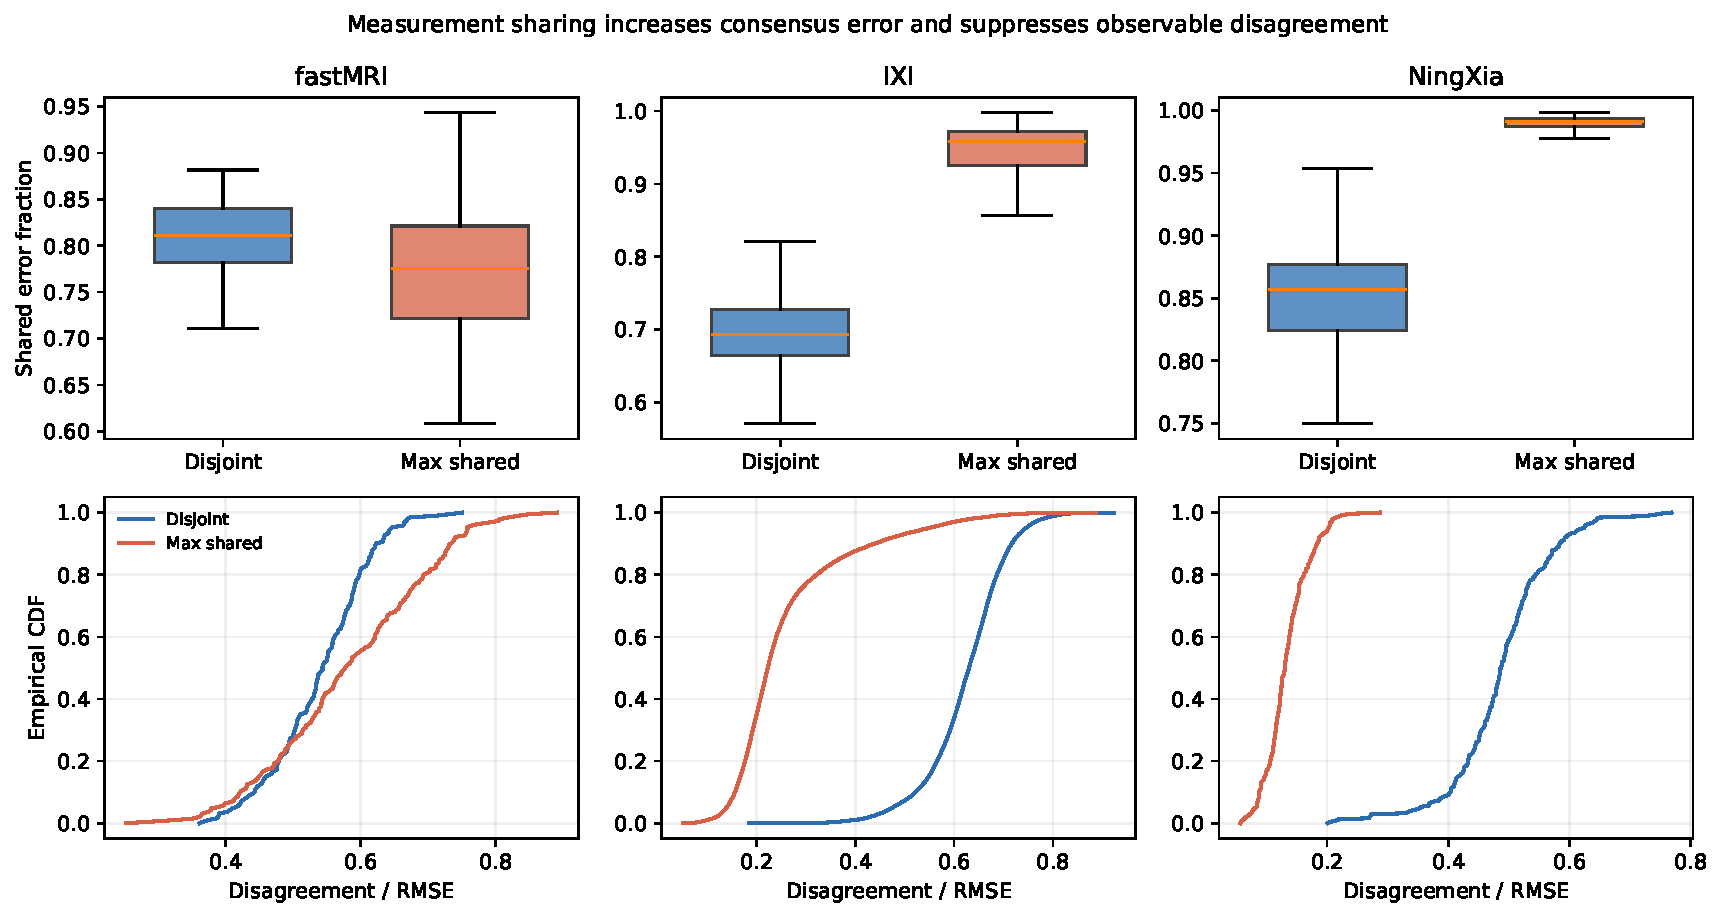
\includegraphics[width=\columnwidth]{p6_e02_consensus_distributions.pdf}
\caption{Plan6 consensus-error characterization. Distribution summaries show shared and observable fractions and their relation to normalized disagreement across measurement-disjoint and maximal-shared contexts. Points retain the model, plane, examination, and patient hierarchy used in inference.}
\label{fig:consensus}
\end{figure}

\subsection{Controlled Measurement-Overlap Intervention}
Figure~\ref{fig:main} and Table~\ref{tab:main} report the primary comparison. On fastMRI, zero-overlap disagreement had plane-level Spearman $\rho=0.960$ with phase-0 MAE, versus 0.605 for the maximal-overlap reversal control, a difference of 0.355 (case-clustered 95\% CI, 0.225--0.557). On NingXia, the corresponding values were 0.891 and 0.699, a difference of 0.193. Correct resampling of eight patient groups gave a 95\% CI of 0.113--0.336. Endpoint differences were exactly zero because both scores were evaluated against the same stored phase-0 error.

\begin{figure}[t]
\centering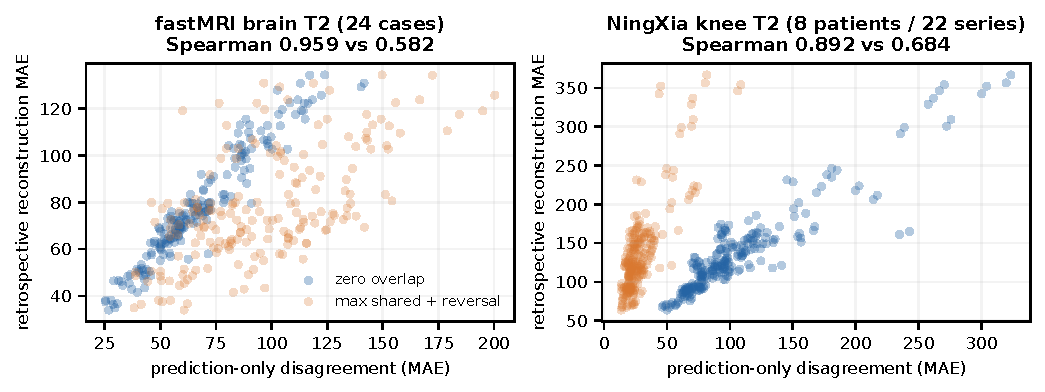
\includegraphics[width=\columnwidth]{fig3_main_overlap.pdf}
\caption{Same-target controlled result. Each point is a model--plane observation; inference is clustered by case (fastMRI) or patient (NingXia). Zero-overlap scores rank retrospective MAE better than the shared-anchor reversal control.}
\label{fig:main}
\end{figure}

\begin{table}[t]
\caption{Zero versus maximal shared-anchor reliability}
\label{tab:main}\centering
\begin{tabular}{p{1.1cm}p{1.0cm}rrrr}
\toprule
Cohort & Model & $\rho_0$ & $\rho_{\max}$ & $\Delta\rho$ & 95\% CI \\
\midrule
fastMRI & pooled & .960 & .605 & .355 & [.225,.557] \\
 & HAT & .967 & .626 & .340 & [.205,.559] \\
 & SwinIR & .958 & .582 & .375 & [.233,.586] \\
NingXia & pooled & .891 & .699 & .193 & [.113,.336] \\
 & HAT & .892 & .764 & .128 & [.025,.233] \\
 & SwinIR & .890 & .632 & .258 & [.133,.513] \\
\bottomrule
\end{tabular}
\end{table}

\subsection{Three-Cohort Multi-Endpoint Robustness}
The frozen two-cohort comparison in Table~\ref{tab:main} used every eligible plane and remains a historical audit target. Plan6 added an independently scripted, common three-plane-per-examination evaluation so IXI could enter the same experiment without altering the original files. In that evaluation, mean architecture-pooled MAE-ranking advantages were 0.117 on fastMRI, 0.086 on IXI, and 0.185 on NingXia (Table~\ref{tab:endpoints}). Each architecture and cohort retained the expected direction. The smaller Plan6 differences relative to the historical all-plane analysis reflect fixed plane sampling and a common endpoint implementation, not model retraining.

All 42 combinations of three cohorts, two architectures, and seven endpoints had a positive disjoint-minus-shared rank-correlation difference (Fig.~\ref{fig:metrics}). The effect therefore did not depend on selecting MAE after observing the results. Intensity endpoints were the most stable: architecture-pooled differences for MAE/RMSE/MSE were 0.117/0.193/0.151 on fastMRI, 0.086/0.083/0.082 on IXI, and 0.185/0.210/0.210 on NingXia. Low-frequency MAE behaved similarly (0.123/0.103/0.198). Gradient and high-frequency endpoints also favored disjoint contexts on average, but several smaller-cohort architecture-specific intervals crossed zero.

SSIM-derived error is the important boundary. Absolute SSIM-error correlations were close to zero on fastMRI and negative on NingXia for both contexts, even though the directional difference remained positive. Only IXI gave consistently positive structural-error ranking and intervals excluding zero. A pixelwise absolute-disagreement score therefore exposes broadly poor intensity reconstruction, but it is not a universal surrogate for structural similarity. We retain all endpoints and reject an endpoint-invariant reliability claim.

\begin{table}[t]
\caption{Architecture-pooled Plan6 ranking correlations}
\label{tab:endpoints}\centering\scriptsize
\begin{tabular}{llrrr}
\toprule
Cohort & Endpoint & $\rho_{\rm dis}$ & $\rho_{\rm shared}$ & $\Delta\rho$\\
\midrule
fastMRI & MAE / RMSE & .957/.936 & .840/.743 & .117/.193\\
 & SSIM / gradient & .006/.640 & $-.070$/.423 & .076/.217\\
 & low / high frequency & .960/.562 & .836/.372 & .123/.189\\
IXI & MAE / RMSE & .977/.972 & .891/.888 & .086/.083\\
 & SSIM / gradient & .417/.973 & .081/.908 & .336/.065\\
 & low / high frequency & .975/.969 & .872/.891 & .103/.079\\
NingXia & MAE / RMSE & .862/.807 & .676/.597 & .185/.210\\
 & SSIM / gradient & $-.240$/.629 & $-.326$/.468 & .086/.161\\
 & low / high frequency & .864/.642 & .666/.479 & .198/.164\\
\bottomrule
\end{tabular}
\end{table}

\begin{figure}[t]
\centering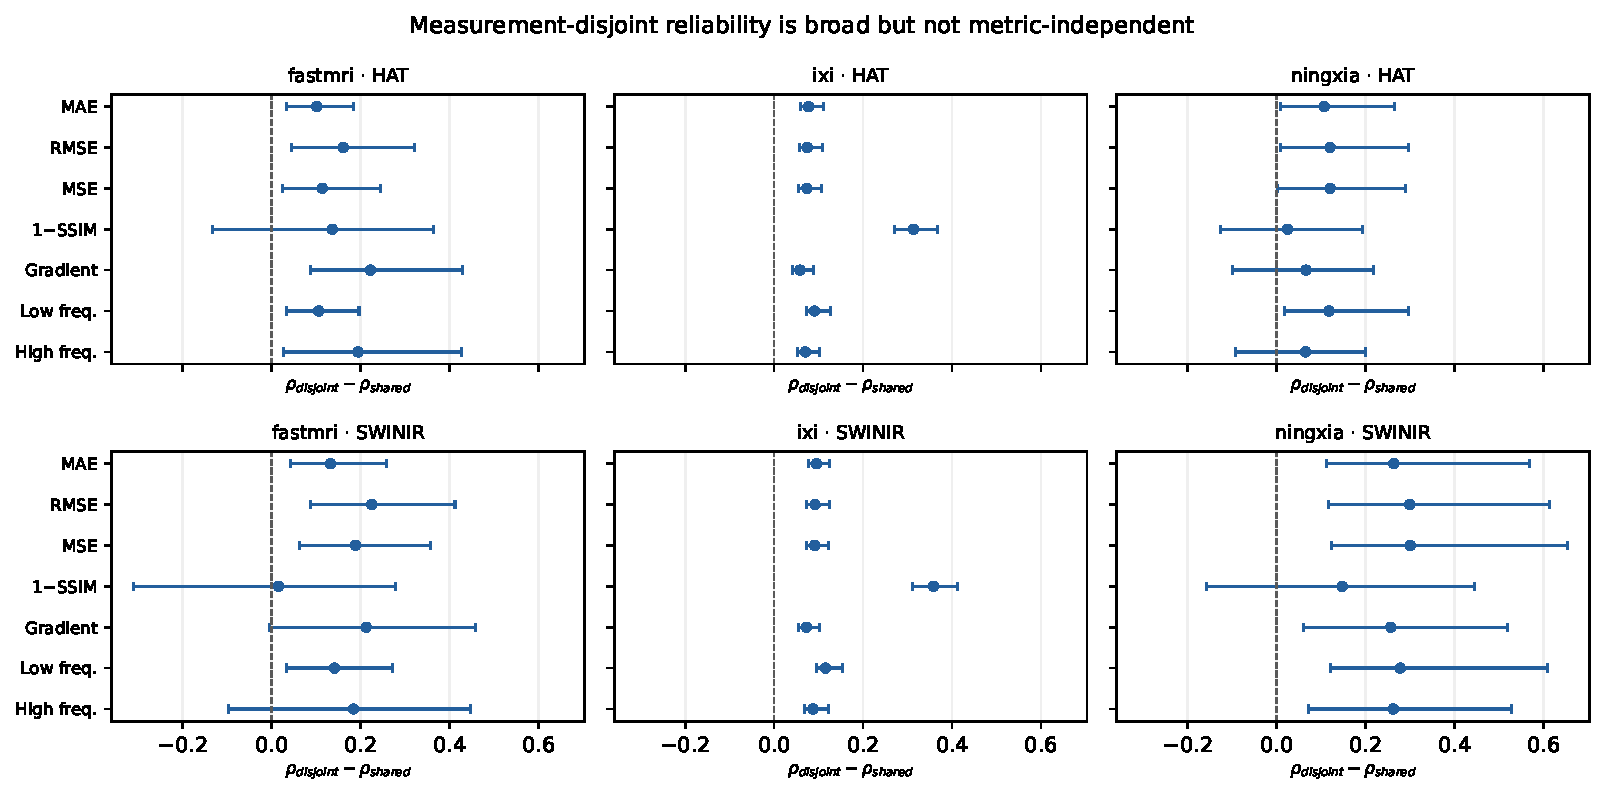
\includegraphics[width=\columnwidth]{p6_e01_metric_robustness.pdf}
\caption{Seven-endpoint robustness. Intervals are clustered by examination for fastMRI/IXI and by patient for NingXia. Every point estimate favors measurement-disjoint disagreement; structural and high-frequency boundaries are visible rather than suppressed.}
\label{fig:metrics}
\end{figure}

\subsection{Architecture and Analytical Generalization}
The effect was positive for HAT and SwinIR separately in both cohorts (Table~\ref{tab:main}; Fig.~\ref{fig:generalization}a). Under zero-overlap grids, classical linear and cubic interpolation also produced strong case-level reliability: Spearman correlations were 0.977 and 0.974 on fastMRI and 0.958 and 0.967 on NingXia (Fig.~\ref{fig:generalization}b). These analytical results show that the useful witness is not uniquely tied to neural stochasticity. Because the analytical experiment lacked a frozen matched maximal-overlap comparator, it supports disjoint-context generality rather than the overlap contrast itself.

\begin{figure}[t]
\centering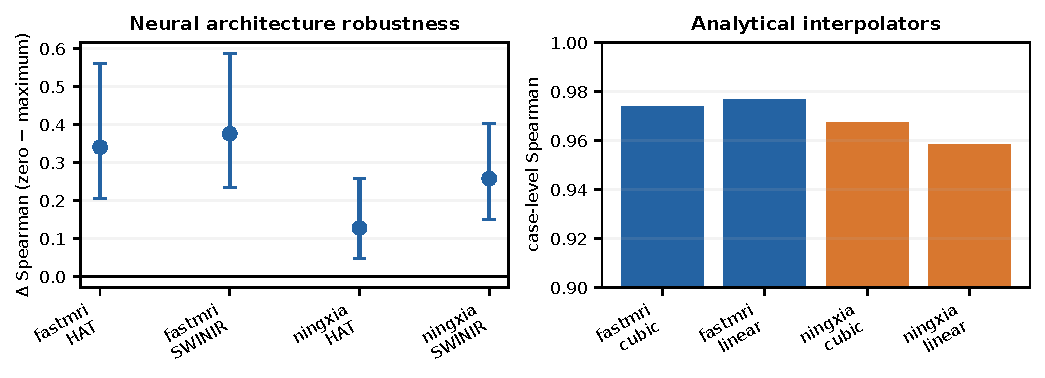
\includegraphics[width=\columnwidth]{fig4_generalization.pdf}
\caption{Generalization. (a) Architecture-specific zero-minus-maximal rank-correlation differences. (b) Case-level disjoint-context correlation for linear and cubic interpolation. Historical NingXia neural intervals were recomputed by eight patient clusters.}
\label{fig:generalization}
\end{figure}

\subsection{Raw Diversity Is Not Sufficient}
On fastMRI, zero-overlap median raw disagreement was only 59.1\% (HAT) and 77.2\% (SwinIR) of maximal-overlap disagreement, yet its error ranking was substantially stronger. Thus a condition can produce larger output differences while being a worse reliability ranker. NingXia showed the opposite magnitude ordering, so raw scale is cohort dependent. The conclusion is deliberately narrow: larger raw output diversity is neither necessary nor sufficient for better ranking in these controls.

\subsection{Analytical Factor Response from $\times2$ to $\times6$}
The analytical factor experiment asks whether consensus blindness strengthens as through-plane information becomes sparser without relying on neural architecture behavior. Figure~\ref{fig:factors} and Table~\ref{tab:factors} show a monotone response in all three cohorts. Mean paired MAE rose from 112.1 to 151.8 on fastMRI, 49.8 to 82.8 on IXI, and 157.1 to 214.6 on NingXia. At the same time, shared fraction rose from 0.843/0.750/0.860 at $\times2$ to 0.953/0.923/0.953 at $\times6$. Observable fraction therefore contracted by factors of 3.38, 3.24, and 2.99, respectively.

Most importantly, the disagreement--error relationship weakened monotonically. Spearman correlation fell from 0.955 to 0.798 on fastMRI, 0.961 to 0.947 on IXI, and 0.937 to 0.818 on NingXia. Absolute disagreement simultaneously decreased on fastMRI and NingXia even though paired error increased. IXI showed a small $\times6$ disagreement rebound (45.2 to 46.6) without reliability recovery. This decoupling is the expected failure mode of raw diversity: a score can become smaller because errors become more aligned, not because images become more accurate.

The factor manipulation changes both missing distance and the target population of eligible planes. We therefore interpret it as an operating-range response, not an isolated causal effect of one extra millimeter. Its strength lies in the repeated pattern across two analytical estimators and all three cohorts. It also establishes that consensus blindness is not produced solely by frozen HAT/SwinIR checkpoints.

\begin{table}[t]
\caption{Analytical factor response (architecture-pooled)}
\label{tab:factors}\centering
\begin{tabular}{llrrr}
\toprule
Cohort & Metric & $\times2$ & $\times4$ & $\times6$\\
\midrule
fastMRI & paired MAE &112.1&137.6&151.8\\
 & shared fraction &.843&.940&.953\\
 & reliability $\rho$ &.955&.833&.798\\
IXI & paired MAE &49.8&67.4&82.8\\
 & shared fraction &.750&.886&.923\\
 & reliability $\rho$ &.961&.947&.947\\
NingXia & paired MAE &157.1&186.2&214.6\\
 & shared fraction &.860&.933&.953\\
 & reliability $\rho$ &.937&.830&.818\\
\bottomrule
\end{tabular}
\end{table}

\begin{figure}[t]
\centering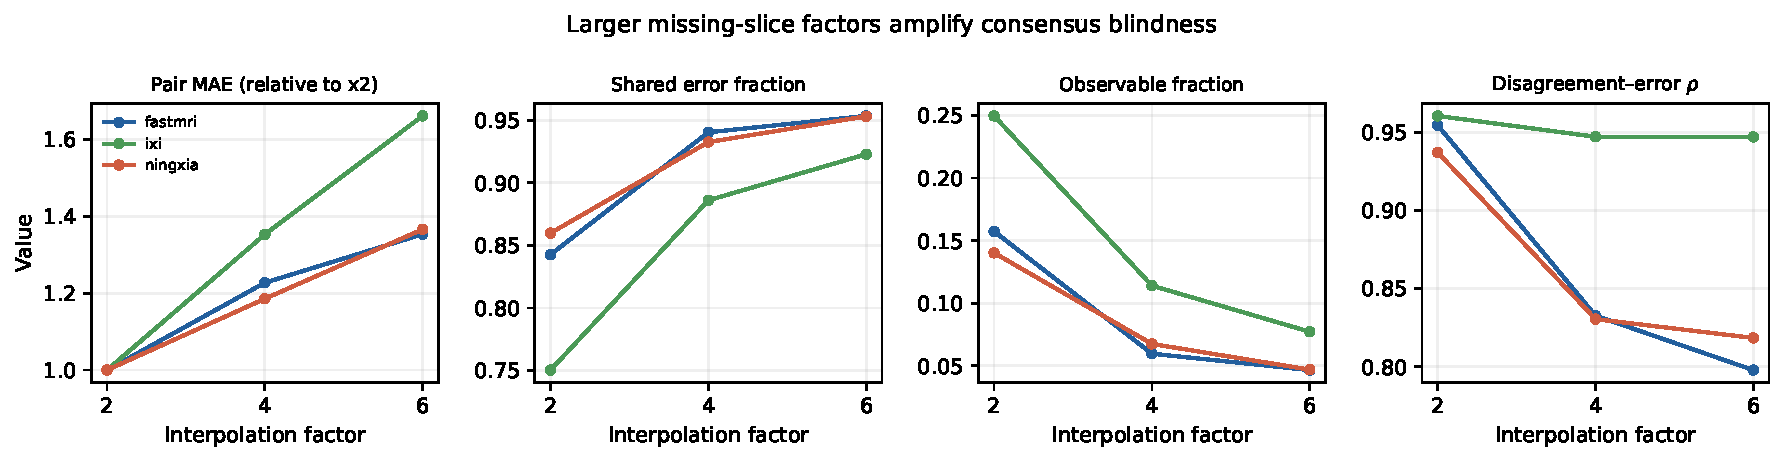
\includegraphics[width=\columnwidth]{p6_e11_factor_robustness.pdf}
\caption{Three-cohort analytical factor response. Increasing factor raises paired error and shared fraction while reducing observable fraction and disagreement--error reliability. Lines connect registered cohort summaries, not repeated-measure causal trajectories.}
\label{fig:factors}
\end{figure}

\subsection{Physical Geometry and Intensity Operating Range}
Before attributing score differences to measurement dependence, we audited the physical correspondence used to pair predictions and targets. Across 322 stored $\times4$ HAT/SwinIR output volumes (48 fastMRI, 230 IXI, and 44 NingXia), prediction and target shapes, NIfTI orientations, and affines were identical. Maximum affine-element difference was zero. Maximum plane-normal angle discrepancy was $1.48\times10^{-6}$ degrees, and maximum matched-plane distance was zero. Every plane match was unchanged for tolerances from $10^{-6}$ to $10^{-1}$ mm. The overlap result is therefore not a by-product of tolerance choice or off-by-one physical plane pairing.

Intensity transformations require a more restrictive conclusion. Under raw stored scale, committee disagreement correlated with examination error at 0.923, 0.957, and 0.874 on fastMRI, IXI, and NingXia. Applying one pooled robust affine transform per case to predictions and target preserved a positive disjoint-minus-shared contrast in all six architecture--cohort strata (0.121--0.700). It did not preserve examination ordering: score-rank correlation with raw scale was 0.797 on fastMRI but $-0.231$ on IXI and 0.637 on NingXia. Separate output normalizations altered ranks further and break the meaning of an absolute paired residual.

Two conclusions follow. First, the within-case directional measurement-overlap effect survives a fair common transform. Second, cross-examination triage depends on the clinically or physically chosen intensity scale. The valid operating range is raw common scale or one transform applied identically to all compared outputs and target. Independently rescaling outputs before disagreement is not a robustness test; it removes amplitude information differently from each reconstruction.

\begin{figure}[t]
\centering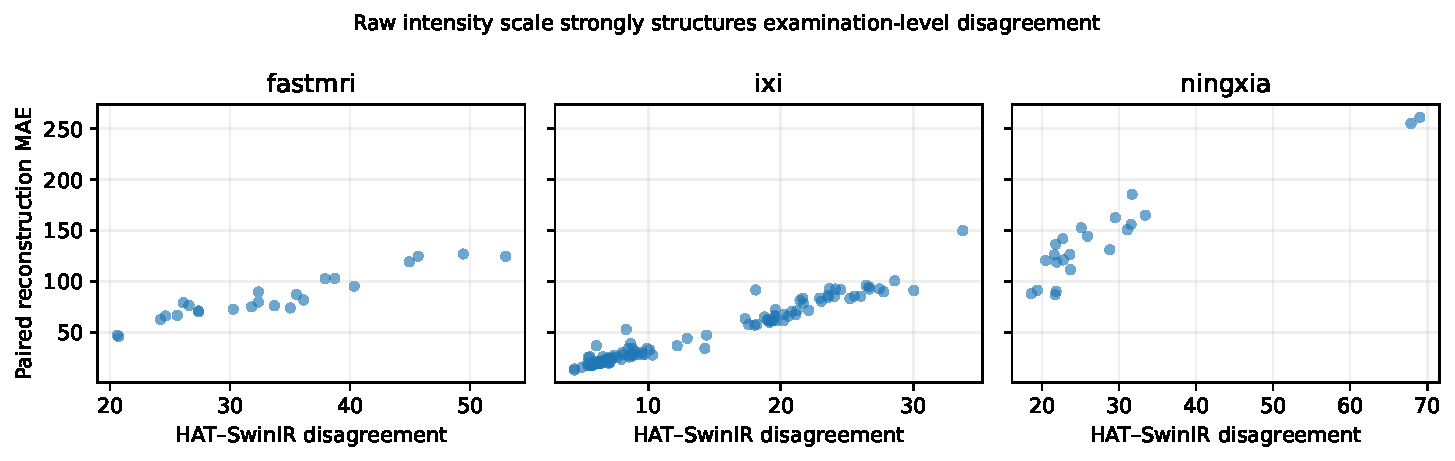
\includegraphics[width=\columnwidth]{p6_e03_intensity_audit.pdf}
\caption{Intensity sensitivity. A shared per-case transform preserves the directional overlap contrast but can change examination ranks; independent output normalization is not a valid calibrated discrepancy operation.}
\label{fig:intensity}
\end{figure}

\subsection{Complete Examination-Level Risk--Coverage}
The central deployment-facing question is not merely whether two continuous variables correlate, but whether rejecting high-score examinations lowers retained reconstruction error. We used one independently stored common endpoint---mean HAT/SwinIR $\times4$ examination MAE---and compared measurement-disjoint, maximal-shared, HAT--SwinIR committee, and adjacent-anchor MAE scores. Figure~\ref{fig:risk} shows all empirical coverage levels; Table~\ref{tab:risk} gives normalized AURC.

Measurement-disjoint disagreement had nAURC 0.0119, 0.0013, and 0.0107 on fastMRI, IXI, and NingXia, respectively. It substantially improved over maximal-shared disagreement (0.0684/0.0139/0.0306) and committee disagreement (0.0193/0.0140/0.0504) in every cohort. The conclusion is not that output disagreement is universally best: adjacent-anchor MAE was weaker on fastMRI and IXI (0.0212/0.0143) but stronger on NingXia (0.0070). Measurement disjointness is supported as the most reliable tested \emph{output-based} construction, while a no-inference acquired-data baseline remains competitive and cohort dependent.

The pattern is consistent across the prespecified 10/20/30/50/70/90\% coverages and is not created by a single rejection threshold. Because the endpoint averages the two architectures while each committee score uses their difference, architecture-independent case difficulty can inflate committee agreement. Indeed, HAT--SwinIR case-error ranks were 0.989, 1.000, and 0.997 across the three cohorts, and examination identity explained 99.1\%, 99.99\%, and 99.78\% of the two-architecture squared-error variation. Two accurate-looking architectures can thus share nearly the same examination ordering while their output difference remains an incomplete witness.

\begin{table}[t]
\caption{Three-cohort selective-risk summary (nAURC; lower is better)}
\label{tab:risk}\centering
\begin{tabular}{lrrr}
\toprule
Score & fastMRI & IXI & NingXia\\
\midrule
Measurement-disjoint & .0119 & .0013 & .0107\\
Maximal-shared & .0684 & .0139 & .0306\\
HAT--SwinIR committee & .0193 & .0140 & .0504\\
Adjacent-anchor MAE & .0212 & .0143 & \textbf{.0070}\\
\bottomrule
\end{tabular}
\end{table}

\begin{figure}[t]
\centering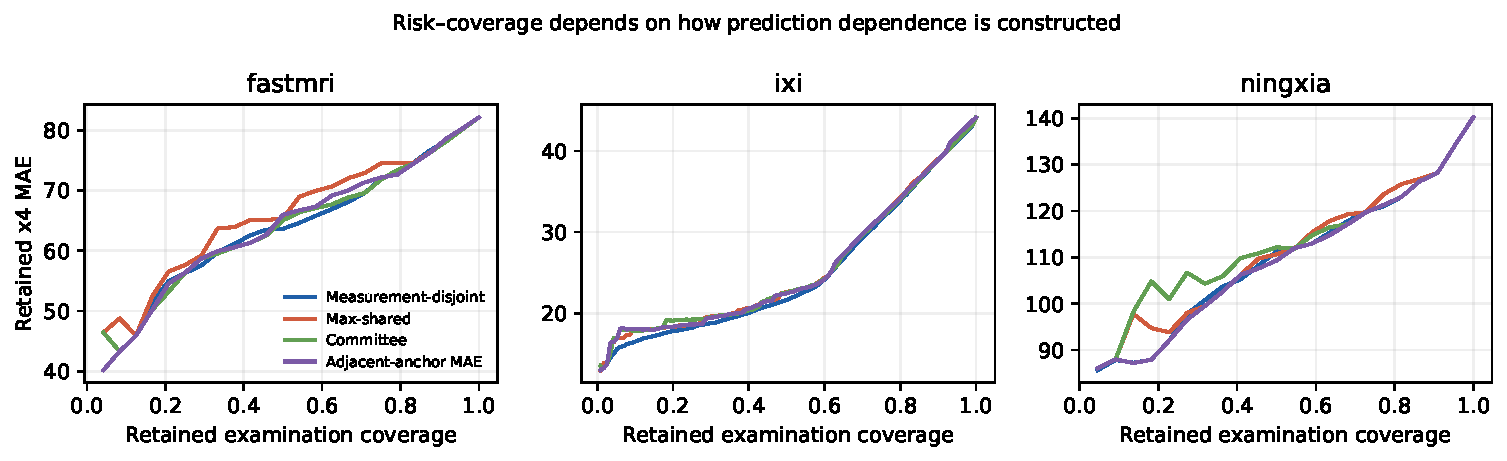
\includegraphics[width=\columnwidth]{p6_e12_risk_coverage.pdf}
\caption{Complete examination-level risk--coverage curves against one stored HAT/SwinIR mean-MAE endpoint. Measurement-disjoint output disagreement beats dependence-preserving output scores in all cohorts; adjacent-anchor MAE is strongest on NingXia.}
\label{fig:risk}
\end{figure}

\subsection{Retrospective Densification Consequence}
The original all-plane consequence analysis found that disjoint $\times4$ disagreement predicted stored same-family $\times4\rightarrow\times2$ MAE reduction on fastMRI ($\rho=0.811$, case-clustered 95\% CI 0.592--0.904) and NingXia ($\rho=0.626$, patient-clustered 95\% CI 0.200--0.844). At a top-25\% budget, selected reductions were 33.36 versus 21.37 for random selection on fastMRI and 35.39 versus 24.25 on NingXia. This analysis preceded the three-cohort rule and is retained as historical evidence, not the Plan6 confirmation.

Plan6 prospectively froze an IXI $\times2$ inference checkpoint, SHA-256, endpoint, and four budgets before generating any of the 115 IXI test outputs. The selected checkpoint was the lowest validation-loss eligible model (validation loss 0.002840859; SHA-256 beginning \texttt{8C87AC89}) and produced a mean I3Net $\times2$ MAE of 12.92, PSNR 35.08 dB, and SSIM 0.953. Anchor-CV score correlated with realized case-level benefit at 0.871 on fastMRI and 0.948 on IXI. Adjacent-anchor MAE gave 0.846/0.950 and output PC gave 0.843/0.970. Every score had positive cluster-bootstrap gain over random at 10, 20, 30, and 50\% budgets. For Anchor-CV on IXI, oracle-normalized gains were 0.920, 0.936, 0.972, and 0.973.

This consequence is deliberately secondary. IXI benefit subtracts frozen I3Net $\times2$ error from the mean frozen HAT/SwinIR $\times4$ error. It tests whether examination difficulty predicts improvement under a denser, separately frozen estimator, not a same-model treatment effect. The union of two disjoint $\times4$ contexts may itself consume measurements approaching denser coverage. Neither analysis validates an online policy that decides which patient to rescan.

\begin{figure}[t]
\centering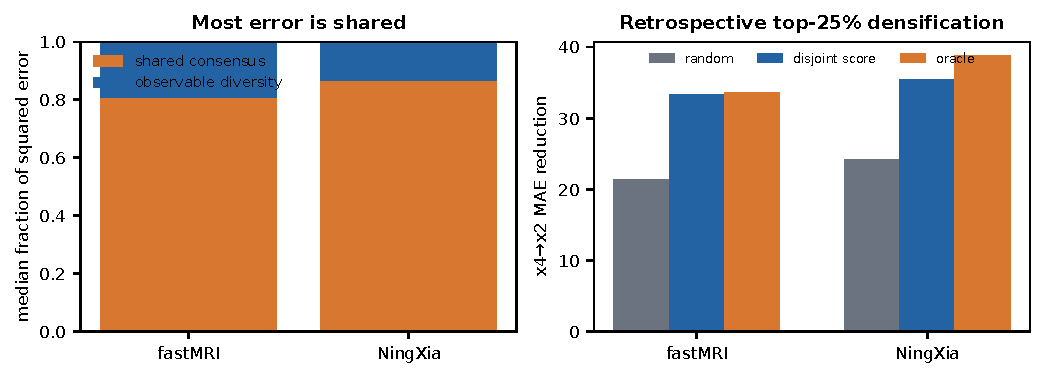
\includegraphics[width=\columnwidth]{fig5_decomposition_consequence.pdf}
\caption{Historical error decomposition and retrospective consequence. These frozen two-cohort results are retained for provenance; the three-cohort energy distributions and Plan6 IXI+fastMRI confirmation are reported separately.}
\label{fig:decomp}
\end{figure}

\subsection{Failure Boundary and Negative Results}
Agreement is not a correctness certificate, but a useful counterexample need not be common. Under the strict Plan6 definition (pooled top-quartile plane MAE and bottom-quartile disagreement), disjoint contexts produced zero stable-wrong planes in all six architecture--cohort strata. Maximal-shared contexts produced none on fastMRI, 0.28--0.32\% on IXI, and 2.42--3.23\% on NingXia. IXI HAT had a paired increase of 0.324 percentage points with clustered CI 0.014--0.865; the other intervals included zero, and the eight-patient NingXia intervals extended to 6.6--8.8\%. The event is mechanistically coherent but too rare and imprecise to present as a high-prevalence clinical failure.

Granularity matters. Examination-level scores summarize expected difficulty but do not identify which interpolated plane is worst. Historical localization found 14 NingXia planes simultaneously in the lowest PC quartile and highest error quartile; 12 occurred at the first generated $\times4$--$\times6$ position, suggesting shared boundary-context failure. Controlled common blur similarly reduced variation while preserving error. These analyses motivate a taxonomy rather than a binary ``works/fails'' statement: (i) stable-wrong consensus, (ii) benign diversity where outputs differ without high target error, (iii) boundary-sensitive error, and (iv) global examination difficulty shared across methods.

Input-side difficulty also had a mixed interpretation. Adjacent-anchor RMSE predicted raw error across fastMRI ($\rho=0.719$), NingXia ($\rho=0.780$), and IXI ($\rho=0.982$ across six methods), but correlations with range-normalized error fell to 0.503, 0.465, and 0.251. A fully normalized feature was robust only on IXI ($\rho=0.644$). A curvature--spacing model improved held-out fastMRI prediction over spacing alone, but absolute transfer to NingXia failed. These negative results reject a universal input-only error law.

Finally, PC beat flip-TTA in all nine frozen fastMRI profiles (mean $\Delta$nAURC $=-0.034$, case-clustered permutation $p=0.0035$). Although all nine NingXia point estimates favored PC, correcting the independent unit to eight patients changed the mean difference to $-0.047$ with $p=0.742$. We therefore do not claim statistically supported PC superiority on NingXia, nor superiority over arbitrary perturbation families.

\subsection{Computational Cost and Information Cost}
Reliability constructions consume different resources and therefore answer different operational questions. On one deterministic representative examination per cohort, Anchor-CV acquired-only scoring required no neural reconstruction and took median 0.42/3.97/3.93 ms on CPU for fastMRI/IXI/NingXia. Adjacent difference cost 0.69/4.00/5.24 ms. Output PC scoring itself took only 1.06/10.20/11.63 ms, but only after two predicted volumes existed.

Committee, flip-TTA, and disjoint-phase strategies each required two neural calls. Measured sequential totals were 0.25--0.29 s on fastMRI, 2.43--3.20 s on IXI, and 0.49--0.60 s on NingXia. Peak allocated GPU memory was approximately 271 MiB for HAT, and paired output storage ranged from 8.6 to 66.5 MiB. Timing used an RTX 5090 D v2, one warm-up and three GPU repetitions; CPU score medians used 100 repetitions. These are representative engineering measurements rather than population estimates.

Compute cost is not acquisition cost. A disjoint phase score requires a different set of physical anchors, whereas committee/TTA can reuse the same acquired scan. Anchor-CV and adjacent difference use acquired anchors only but summarize input difficulty rather than direct reconstruction inconsistency. The appropriate comparison therefore has two axes: predictive reliability and which information must be acquired or generated. The efficiency result supports Anchor-CV as inexpensive, not as more accurate than every baseline.

\subsection{Reproducibility and Evidence Separation}
Each Plan6 experiment writes a machine-readable per-observation table, a summary table, a JSON manifest, and a figure from the same records. The geometry audit records every output path and correspondence check. The IXI $\times2$ evaluation records the checkpoint hash and all 115 output identities. No result was copied from a plot. Historical frozen results and newly registered Plan6 results retain separate prefixes so a revised script cannot silently overwrite earlier evidence.

The TMI and CVPR evidence scopes are also separated. This manuscript uses physical measurement overlap, error-energy distributions, endpoint/factor robustness, geometry/intensity controls, and risk--coverage. The conference paper uses finite-difference neural influence and an acquired-anchor score to study a finer local mechanism. Shared data are disclosed, but the principal hypotheses and tables are not interchangeable. This separation prevents a single exploratory analysis from being counted twice as independent confirmation.

\section{Discussion}
The experiments support a mechanistic account of disagreement blindness in deterministic MRI interpolation. Reconstruction contexts can share a large consensus error, and Eq.~\eqref{eq:cov} shows why aligned errors disappear under subtraction. The controlled phase-grid intervention changes the acquired information supporting the same target. Disjoint grids rank error better than a same-anchor reversal context across two anatomies and two neural architectures, while analytical interpolation provides an estimator-family replication. The result is stronger than observing that perturbations produce different outputs: the paired endpoint is fixed, measurement identity is recorded, and a raw-magnitude control demonstrates that more output variation is not itself the operative goal.

The findings also clarify what disagreement can and cannot mean. High disjoint-context disagreement is useful evidence of context-sensitive failure. Low disagreement is ambiguous because both contexts may share bias. In practice, reliability systems should therefore seek contexts that reduce dependence in error-generating information, while retaining explicit stable-wrong safeguards. This principle complements probabilistic reconstruction: even posterior or ensemble samples can underestimate risk if their construction does not vary the source of shared error.

This perspective separates three properties that are often conflated. \emph{Diversity} is the observed distance between outputs. \emph{Observability} is the fraction of actual paired error that survives in that distance. \emph{Calibration} maps a score to a probabilistic or absolute error statement. Our experiments address the first two and show that diversity alone does not determine observability; they do not establish the third. Consequently, a disjoint-context score can rank difficult examinations while remaining unsuitable for statements such as ``this slice has less than a specified error.''

The retrospective densification result offers a methodological consequence. Cases with larger disjoint disagreement tended to realize larger gains from denser stored sampling. That relationship is promising for acquisition-allocation research because the score itself uses only alternative sparse contexts. However, constructing two disjoint $\times4$ grids consumes the union of measurements equivalent to denser coverage in this simulation. A practical policy would require a lower-cost pilot, sequential sampling, or a pre-inference surrogate evaluated prospectively. The present study does not solve that deployment problem.

The controlled intervention also has an imaging-specific interpretation. Through-plane anchors are not exchangeable generic augmentations: their physical locations determine both interpolation distance and the anatomical information available to a reconstruction. Preserving the physical target and evaluation support while recording anchor identity is therefore necessary for assigning a measurement-overlap interpretation. This requirement explains why ordinary flip-TTA, architecture committees, and phase-grid comparisons answer related but nonidentical reliability questions.

IXI now supplies the largest replication of the overlap, distribution, metric, factor, and selective-risk analyses. Its contribution is not only statistical precision. IXI differs in volume depth and intensity distribution from fastMRI and supplies many more eligible physical planes, yet the direction of every endpoint contrast and the analytical factor trend persisted. At the same time, IXI exposes the intensity-normalization boundary particularly clearly: common per-case scaling preserved the overlap contrast while substantially changing examination ranks. Replication therefore supports the physical-dependence mechanism without implying a universal absolute scoring scale.

\subsection{What Is and Is Not Novel}
The identity in Eq.~\eqref{eq:cov}, correlated ensemble errors, systematic-error blindness, and leave-one-slice-out interpolation evaluation all predate this study \cite{brown2005diversity,hu2021predict,horvath2017highorder}. The contribution that survives the literature audit is their task-specific connection to an auditable physical cause and a paired intervention: predictions for the same missing MRI plane can reuse known acquired slices, and this reuse changes error observability. Three-cohort endpoint/factor characterization, physical-plane auditing, strict failure prevalence, and selective-risk consequences make that connection falsifiable.

This positioning is intentionally narrower than claiming a new theory of uncertainty. It is also different from proposing another network or uncertainty head. A new head can improve calibration yet still inherit shared acquisition bias; a measurement-disjoint comparison can reveal context-sensitive error yet remain uncalibrated. The methods are complementary. A promising future design would combine physically diverse contexts with conformal or held-out calibration, then test whether coverage remains valid under acquisition and anatomy shifts.

\subsection{Implications for Reliability-System Design}
The results suggest a hierarchy of design checks. First, define the physical target and record exactly which measurements support each prediction. Second, measure dependence at the information level rather than count output transforms. Third, choose an endpoint aligned with the intended harm; MAE disagreement did not reliably rank SSIM error in two cohorts. Fourth, evaluate complete risk--coverage curves and strong acquired-data baselines. Fifth, keep a stable-wrong safeguard because no amount of consensus is a correctness certificate.

The hierarchy changes how negative results should be read. The NingXia adjacent-anchor result does not refute measurement dependence; it shows that a simple input-difficulty score can outperform all tested output scores in a small external knee cohort. The rare stable-wrong rate does not make the algebra irrelevant; it constrains the frequency of one extreme phenotype under one definition. The IXI normalization reversal does not erase the paired contrast; it prohibits careless cross-examination calibration. These boundaries are useful outcomes because each identifies a separate engineering requirement.

\subsection{Alternative Explanations}
The maximal-shared reversal changes ordering as well as anchor identity, so order equivariance is a possible contributor. However, four observations argue against an order-only account of the full evidence: the consensus-fraction relation holds within both contexts after error/examination control; the analytical factor response uses no learned ordering sensitivity; all endpoint contrasts retain one direction across both architectures; and raw disagreement magnitude does not track ranking quality. These observations do not isolate a pure causal coefficient for overlap, but they support measurement dependence as a coherent common explanation.

Case difficulty is another alternative. The nearly perfect HAT--SwinIR case-error agreement shows that anatomy, contrast, spacing, and other examination properties dominate between-case error variation. The partial distribution analysis explicitly controls examination identity, and the target-preserving contrast pairs the same plane. Thus common difficulty explains why all methods struggle on similar cases, whereas measurement dependence explains how much of paired error remains visible after subtraction. Both phenomena coexist.

Finally, results might reflect intensity range alone. Raw range clearly matters for case triage, and separate normalization can distort the score. Yet applying one common robust transform to predictions and target preserved the disjoint advantage in every dataset--architecture stratum. Hence dynamic range contributes to absolute ordering but does not fully explain the paired direction.

\subsection{Clinical Interpretation}
No score in this work should be displayed as a probability of diagnostic correctness. The endpoints are image-domain fidelity measures and no radiologist reader study was performed. A low score means only that the tested contexts agree under the stated scale; it cannot exclude a common hallucination, smoothing loss, or pathology omission. A high score can flag a case for review, but it cannot identify which output or anatomical structure is wrong.

A clinically meaningful follow-up would predefine an action: retain the original thick-slice series, request an additional acquisition, route the case to a human reader, or suppress an interpolated view. The chosen action determines the acceptable error endpoint and coverage. Such a study should be prospective, include pathology-enriched strata, account for the cost and feasibility of acquiring alternate anchors, and measure downstream decisions rather than only MAE. The current evidence justifies that next experiment; it does not substitute for it.

\section{Limitations}
All phase grids are retrospective simulations from dense volumes; no scanner prospectively changed its sampling. Although three cohorts enter all structurally eligible Plan6 analyses, NingXia has only eight independent patient groups despite 22 series, and all data are T2 weighted. Only HAT and SwinIR support the decisive neural phase-grid experiment; I3Net was infeasible without artificial padding. The maximal-overlap reversal control changes through-plane ordering and may invoke equivariance effects beyond overlap. A strict multi-level overlap ladder with fixed two-anchor distances is geometrically infeasible; the analytical factor study changes distance and target availability together.

Intensity-derived MAE and disagreement require comparable preprocessing within each paired profile and do not support cross-cohort absolute calibration. The strong case component means correlations partly reflect examination difficulty even when plane pairing is exact. The study has no reader task, pathology label, clinical endpoint, prospective adaptive acquisition, or safety analysis. It cannot identify which output is wrong, guarantee accuracy from agreement, or establish universal superiority over uncertainty estimators. Common-mode blur and boundary failures remain explicit counterexamples. Stable-wrong prevalence depends on a quartile definition and was low. Finally, parts of the evidence were generated after inspecting earlier results; Plan6 hypotheses were registered before their endpoints were computed, but the work is not a preregistered clinical trial.

The retrospective densification analyses have additional limitations. The historical result uses different model--case units from the Plan6 IXI result; IXI compares a mean two-architecture $\times4$ endpoint with I3Net $\times2$. The score may primarily identify intrinsically difficult cases rather than a treatment interaction with sampling factor. A genuine acquisition-benefit claim requires randomization or a prospective within-model counterfactual. We report only case-level predictive consequence.

\section{Ethics and Data Availability}
fastMRI and IXI are publicly accessible human-derived MRI resources; use here was retrospective and involved locally prepared deidentified images. The exact consent, institutional-review, and data-use wording for the particular fastMRI-brain and IXI releases must be copied from their governing records before submission. NingXia is an internal human MRI cohort. \textbf{[ETHICS INFORMATION REQUIRED FROM AUTHORS: approving or exempting institution, decision/approval identifier where applicable, consent or waiver, and permitted data-use statement.]}

Code, immutable historical experiment records, case-level manifests, and derived numerical outputs are organized in the accompanying repository. Raw public data remain under their source licenses; internal NingXia images are not redistributed. An anonymized repository URL and any sharing restrictions must be supplied before submission. No generative-AI content disclosure is asserted here; authors must add the disclosure required by current IEEE policy if applicable to manuscript preparation.

\section{Conclusion}
In deterministic MRI slice interpolation, disagreement observes differences between reconstruction errors, not error itself. Shared measurements can align errors and conceal them. Across fastMRI, IXI, and patient-clustered NingXia, target-preserving disjoint anchor grids ranked intensity-domain error more effectively than shared-anchor output comparisons. The direction persisted across two neural architectures, seven endpoints, analytical factors $\times2$--$\times6$, exact geometry checks, common-scale perturbations, and complete risk--coverage curves. The boundaries are equally important: structural-error ranking was inconsistent, stable-wrong events were rare but possible, and a simple adjacent-anchor score won on NingXia. The supported principle is narrow: design reliability contexts to reduce shared error-generating information, evaluate them against the intended endpoint, and never interpret agreement as a correctness certificate.

\appendices
\section{Registered Hypotheses and Decision Rules}
This research master preserves the full Plan6 evidence chain. The multi-endpoint hypothesis was confirmed if a majority of justified endpoints favored disjoint contexts in every eligible cohort, with all endpoints disclosed. The consensus-distribution hypothesis required a negative association between shared fraction and normalized disagreement after total-error/examination control. The geometry hypothesis required exact shape/orientation/affine agreement and no sign reversal under small physical matching tolerances. The intensity hypothesis permitted only one common transform applied to all compared arrays. The factor hypothesis required monotone higher shared fraction and lower observable fraction/reliability from $\times2$ to $\times6$ in all cohorts. The risk hypothesis required disjoint disagreement to improve over dependence-preserving output scores but did not require it to beat every acquired-input baseline.

These rules were written before the corresponding Plan6 endpoints were computed. The following outcomes prevent overstatement: SSIM ranking failed to generalize absolutely; independent normalization was rejected; maximal-shared stable-wrong prevalence was low; adjacent MAE beat disjoint disagreement on NingXia nAURC; and the densification analysis remains retrospective. The manuscript treats a negative boundary as evidence about scope rather than removing it from the result set.

\section{Measurement and Matching Definitions}
Let a NIfTI volume have affine $A$ and voxel coordinate $v=(i,j,k,1)^\top$. Physical location is $x=Av$. The slice normal is the normalized third affine column and the signed through-plane coordinate is its dot product with the slice origin. Predictions and targets match only when array shape and orientation agree and the absolute coordinate difference is within tolerance. Plan6 tested $10^{-6}$, $10^{-5}$, $10^{-4}$, $10^{-3}$, $10^{-2}$, and $10^{-1}$ mm; the matched set was invariant.

For an interpolation factor $r$, an anchor lattice with phase $p$ is $\{z:z\equiv p\pmod r\}$. A target plane is eligible only if absent from every compared anchor lattice and bracketed by the measurements required by the estimator. Measurement overlap is computed from physical anchor identities, not array indices after reversal or augmentation. This definition prevents a transformed copy of one acquired slice from being counted as new information.

The deployment mask is derived once from the reference reconstruction used by the registered profile. It is then held identical when calculating disagreement and every target endpoint for a paired contrast. This avoids allowing a poor prediction to select an easier evaluation region. Empty, nonfinite, shape-mismatched, or physically unmatched planes are excluded by deterministic validation before any correlation is calculated; exclusions are written to the manifest rather than repaired with padding.

\section{Additional Statistical Interpretation}
Cluster bootstrap intervals quantify sensitivity to sampling independent examinations or patients, not pixelwise noise. When an eight-patient sample yields a wide interval despite many planes, the interval is doing the intended job: repeated images do not manufacture independent clinical units. The study consequently emphasizes direction consistency and effect ranges instead of interpreting every plane-level $p$ value as confirmatory.

Correlation differences are paired because the disjoint and shared scores target the same endpoint observation. Bootstrap resampling carries both scores, architectures, planes, and endpoints for a cluster together. Partial rank correlations are computed after rank-transforming variables and residualizing shared fraction and disagreement against total error and examination indicators. They describe conditional monotone association; they do not prove causal mediation.

Risk--coverage curves use examination aggregation to align the score with a plausible review unit. If $s_i$ is a score and $e_i$ the stored endpoint, observations are sorted by increasing $s_i$ and $R(k/n)=k^{-1}\sum_{j=1}^k e_{(j)}$. nAURC subtracts oracle area and divides by reverse-oracle minus oracle area. A value near zero means the ranking approaches the best ordering available from the endpoint; it does not mean zero reconstruction risk.

\section{Evidence Inventory}
The multi-endpoint experiment contains 42 primary dataset--architecture--endpoint contrasts. The distribution experiment contains both contexts for every cohort and architecture, per-plane energy components, partial associations, and strict stable-wrong prevalence. The geometry audit covers 322 neural output volumes. The analytical factor experiment covers 144/216/240 planes on fastMRI, 7,334/11,001/12,075 on IXI, and 168/252/220 on NingXia at factors 2/4/6, respectively. The risk experiment covers all 24/115/22 examination or series units, with NingXia inference clustered into eight patients.

Every reported Plan6 result has a source table under \texttt{experiments/}; every displayed figure is generated from those tables. The frozen historical figures remain because they document the sequence of evidence and provide full-plane comparisons that Plan6 did not overwrite. Before external release, anonymous repository identifiers, public-data licenses, internal-data access language, and ethics approval details must replace the bracketed author action in the Ethics section.

\section{Extended Theory and Identifiability}
\subsection{Bias, Variance, and Cross-Context Covariance}
The deterministic identity in Eq.~\eqref{eq:cov} applies observation by observation. A complementary population view clarifies why ordinary diversity can fail even when contexts are produced by different models. Write $e_a=b_a+u_a$ and $e_b=b_b+u_b$, where $b$ is the mean error over a target population and $u$ is a zero-mean deviation. Then
\begin{align}
E\|e_a-e_b\|^2 ={}& \|b_a-b_b\|^2 + {\rm tr}(\Sigma_a)+{\rm tr}(\Sigma_b) \\
&-2{\rm tr}(\Sigma_{ab}). \label{eq:population}
\end{align}
Disagreement misses a shared bias when $b_a\approx b_b$ and is reduced by positive cross-context covariance $\Sigma_{ab}$. Measurement reuse can contribute to both terms: identical anchors can induce a common smoothing direction and common case-dependent deviations. Equation~\eqref{eq:population} does not assert that overlap is the only source. Shared training data, architecture priors, preprocessing, and anatomy can also align errors.

This distinction matters for interpreting the intervention. Integer anchor overlap is an observed design property, not an estimate of ${\rm tr}(\Sigma_{ab})$. The experiment tests whether changing the design property moves empirical observability in the predicted direction. It cannot decompose the exact fraction caused by each anchor, nor infer a structural coefficient without assumptions about ordering, spacing, and model response. The appropriate causal language is therefore ``target-preserving intervention with a residual order confound,'' not ``identified effect of one shared slice.''

\subsection{Four Non-Identifiability Boundaries}
First, two predictions and their disagreement do not identify either individual error. For any observed $(f_a,f_b)$ and arbitrary image $c$, choosing $y=f_a-c$ yields $e_a=c$ and $e_b=c+(f_b-f_a)$. Infinitely many targets produce the same disagreement. No deterministic mapping from $\|f_a-f_b\|$ to exact target error exists without additional distributional or calibration assumptions.

Second, zero disagreement gives no finite upper error bound. Set $f_a=f_b=g$ and choose $y=g+c$ for arbitrarily large $\|c\|$. Then disagreement is zero while both errors grow without bound. The stable-wrong examples are empirical finite-scale instances of this elementary boundary.

Third, large disagreement is only one-sided evidence. By the triangle inequality, $d(f_a,f_b)\le d(f_a,y)+d(f_b,y)$, so at least one of two predictions has error at least $d(f_a,f_b)/2$. The identity does not say which prediction is worse, and it does not guarantee that the stored primary prediction is the inaccurate one. Reliability triage can flag a pair but cannot adjudicate between its members.

Fourth, aggregation can change the estimand. Plane-level Spearman correlation weights examinations with more eligible planes more heavily; examination-level correlation gives every examination one rank. Median aggregation suppresses isolated failures, whereas maximum aggregation is sensitive to a single artifact. We use plane-level analysis for the local overlap mechanism and examination-level medians/means for selective risk. Neither should be silently substituted for the other.

\subsection{Transform Invariance and Its Limits}
A single global affine intensity transform $x\mapsto \alpha x+\beta$, $\alpha>0$, multiplies MAE and disagreement by $\alpha$ and therefore preserves their global ranks. A different transform for every examination multiplies each case by a different $\alpha_i$; within-case plane ranks are preserved, but between-case triage ranks need not be. This explains why the per-case common normalization preserved the direction of the paired overlap contrast yet changed IXI examination ordering.

Independent transformations $a\mapsto\alpha_a a+\beta_a$ and $b\mapsto\alpha_b b+\beta_b$ are more problematic. Their difference includes $(\alpha_a-\alpha_b)y$ and offset terms even when the untransformed errors agree. Conversely, normalizing each output by its own range can remove an amplitude failure that should contribute to absolute error. The Plan6 independent-output condition is included as a falsification control, not a recommended preprocessing scheme.

SSIM adds another transform boundary. Its contrast and structure terms respond differently from pixelwise absolute difference, and the global data range enters its definition. Positive MAE ranking therefore does not mathematically imply positive SSIM-error ranking. The fastMRI/NingXia results demonstrate this distinction empirically and motivate endpoint-specific validation.

\subsection{Expected Response to Increasing Factor}
If interpolation distance grows, marginal errors can increase while both estimators converge toward a similar low-frequency prior. In the decomposition, $T$ rises, $q=S/T$ rises, and $O/T$ falls. Absolute disagreement may rise, fall, or remain unchanged because it depends on the product of total energy and observable fraction. Reliability declines when between-case changes in $O$ cease to track changes in $T$.

The analytical factor result matches this qualitative response in all cohorts. It is not a theorem that every model must behave monotonically: a model trained specifically for larger spacing might change its errors or exploit more context. The value of the experiment is to demonstrate that the predicted failure occurs even in transparent estimators without stochastic sampling or learned uncertainty heads.

\section{Cohort-Specific Evidence Synthesis}
\subsection{fastMRI Brain T2}
fastMRI supplies the smallest public brain test panel but has a clean 24-examination independent unit and extensive historical frozen evidence. In the three-plane Plan6 endpoint experiment, disjoint MAE correlations were 0.964 for HAT and 0.950 for SwinIR, compared with 0.863 and 0.818 for maximal-shared contexts. RMSE differences were larger (0.161 and 0.225), suggesting that measurement dependence is not confined to numerous small residuals. Low-frequency MAE nearly matched overall MAE; gradient and high-frequency endpoints were weaker but remained directionally positive.

The structural boundary is clearest here: SSIM-error correlations were 0.017 and $-0.005$ for disjoint contexts. The shared-context values were also weak or negative. Thus disjoint disagreement can be an excellent intensity-error ranker while providing essentially no SSIM-error ordering on this panel. This is a substantive endpoint mismatch, not merely a wide interval around a strong effect.

fastMRI also gives the largest historical zero-versus-maximal difference: pooled all-plane $\Delta\rho=0.355$ with case-clustered interval 0.225--0.557. The Plan6 common three-plane estimate is smaller because it samples equal physical positions per case. Both results answer legitimate but different questions. The former estimates performance over all available generated planes; the latter emphasizes balanced examination coverage and cross-cohort comparability.

In selective risk, the disjoint score achieved nAURC 0.0119. Committee disagreement had slightly higher Spearman correlation (0.962 versus 0.955) yet worse nAURC (0.0193), illustrating that a global rank statistic and the geometry of the high-risk tail are not identical. At 50\% coverage, disjoint retained risk was 63.65 and equaled the oracle subset, whereas maximal-shared and adjacent scores retained 65.36 and 65.97. The small sample makes individual coverage steps coarse, so the integrated result is emphasized.

The analytical factor response was strong: shared fraction rose by 0.111 from $\times2$ to $\times6$, observable fraction fell from 0.157 to 0.047, and reliability fell by 0.157. This convergence occurred while mean paired error rose by 35\%. It supplies a transparent example of disagreement becoming less informative as reconstruction becomes harder.

\subsection{IXI Brain T2}
IXI is the largest cohort and provides the strongest precision test. It contributes 115 examinations, 7,104 neural model--plane observations per condition in the distribution audit, and more than 7,000 analytical targets even at $\times2$. Every one of the 14 architecture-specific endpoint intervals excluded zero. MAE disjoint correlations were 0.977 for both HAT and SwinIR; maximal-shared correlations were 0.900 and 0.881. SSIM-error was meaningfully rankable only here (0.422/0.412 disjoint versus 0.108/0.053 shared), showing that structural reliability can be dataset dependent rather than impossible in principle.

The consensus relation was especially strong in shared contexts: partial rank correlations between shared fraction and normalized disagreement were $-0.975$ for HAT and $-0.973$ for SwinIR after controlling total error and examination. Strict stable-wrong prevalence remained small (0.324\% and 0.282\%), which separates a strong continuous suppression mechanism from the frequency of an extreme quartile event.

IXI selective risk approached the endpoint oracle. Disjoint nAURC was 0.00126 and Spearman correlation 0.994, compared with nAURC about 0.014 for maximal-shared, committee, and adjacent-anchor scores. At 10\% coverage, disjoint retained risk was 16.58 versus oracle 16.55; at 50\%, both were 21.70. These close numbers should not be generalized to an external IXI deployment because models and reliability analyses share the same development program, but they show that dependence-aware ranking can be nearly optimal on the frozen panel.

IXI also produces the strongest warning about scale. Raw committee-error correlation was 0.957, but a common per-case robust normalization reduced it to 0.256 and reversed the score rank relative to raw scale ($-0.231$). The directional disjoint-minus-shared contrast survived. Hence two claims that might appear contradictory are both true: the within-case mechanism is robust to a fair transform, and the across-case ordering is not invariant to case-specific scaling.

At analytical factors, shared fraction rose $0.750\rightarrow0.886\rightarrow0.923$ and reliability changed $0.961\rightarrow0.947\rightarrow0.947$. The last decrement is small. IXI therefore supports the direction but indicates a possible floor or saturation by $\times4$. Absolute disagreement decreased then rebounded slightly, further demonstrating that raw magnitude is not a monotone proxy for observability.

The frozen $\times2$ I3Net run makes IXI eligible for the two-dataset consequence test with fastMRI. All 115 outputs, corresponding ground truths, sparse inputs, analytical baselines, and metric rows were present before benefit analysis. High benefit correlation across Anchor-CV, adjacent MAE, and output PC indicates that intrinsic case difficulty drives much of the result; it does not distinguish a uniquely causal acquisition score.

\subsection{NingXia Knee T2}
NingXia tests anatomy and provenance transfer but has only eight independent patients. The 22 series and 124 neural model--plane observations per context improve descriptive coverage, not the number of independent clinical units. All bootstrap and selective-risk uncertainty therefore carries series together by patient.

Plan6 MAE correlations were 0.866/0.858 for disjoint HAT/SwinIR and 0.759/0.612 for shared contexts. The effect is larger for SwinIR, but patient-clustered precision is lower. SSIM-error correlation was negative for both conditions and architectures; the positive difference means shared measurements made a poor structural score still worse, not that the disjoint score became useful for SSIM triage.

NingXia has the highest strict stable-wrong prevalence in maximal-shared contexts (2.42--3.23\%), yet its intervals are wide. It also contains the historical boundary-localized cases. Together these observations motivate targeted boundary audits in future work, but they do not establish anatomy-specific pathology. Plane location, shallow volume depth, patient protocol, and model domain shift remain entangled.

The selective-risk boundary is scientifically important. Measurement-disjoint disagreement improves clearly over maximal-shared and committee scores, but adjacent-anchor MAE achieves lower nAURC (0.0070 versus 0.0107). At 10\% coverage their retained risks are nearly identical (87.27 versus 87.19); around 50\%, adjacent MAE is lower (109.30 versus 111.24). A reliability system for this cohort could rationally choose the cheaper acquired-input score. This does not weaken the dependence result against output comparators; it narrows the practical recommendation.

The factor pattern is closer to fastMRI than IXI: shared fraction rises $0.860\rightarrow0.933\rightarrow0.953$, observable fraction falls $0.140\rightarrow0.067\rightarrow0.047$, and reliability falls $0.937\rightarrow0.830\rightarrow0.818$. Mean paired error rises while absolute disagreement falls. Replication in an out-of-fold knee setting argues that the factor phenomenon is not brain-specific.

\section{Threats to Validity and Falsification Logic}
\subsection{Internal Validity}
The main threat is that maximal-shared reversal alters order as well as measurement overlap. We mitigate but cannot eliminate it through paired targets, identical anchor identities, two architectures, the within-context energy analysis, raw-magnitude falsification, and an analytical factor experiment without reversal. A future definitive study should construct contexts with matched distances, ordering, and receptive-field position while varying only physical measurement identity; through-plane geometry makes a multi-level version nontrivial.

Target leakage is another threat. Dense targets are used to create retrospective phase grids and calculate endpoints. The score itself never reads the target, but designing the experiment from a dense volume is not equivalent to having two sparse prospective scans. File-level manifests and target-excluded code paths prevent computational leakage; they cannot create prospective evidence.

Selection can enter through eligible-plane filtering. We require the same target to be absent from both contexts and fully bracketed. This excludes boundaries and favors interior anatomy. Historical boundary analysis demonstrates that excluded or underrepresented positions may be clinically harder. We therefore do not extrapolate plane-level correlations to unbracketed extrapolation.

\subsection{Construct Validity}
``Reliability'' here means monotone ranking of a specified image-domain endpoint or reduced retained error under selective coverage. It does not mean calibration, confidence intervals with nominal coverage, diagnostic correctness, robustness to every domain shift, or user trust. The explicit seven-endpoint panel shows why this distinction matters.

Measurement disjointness is binary in the primary neural contrast. It does not encode how strongly each anchor affects a prediction, whether unshared anchors contain redundant anatomy, or whether training induces a common prior. The separate conference branch studies continuous finite-difference influence; this journal paper intentionally does not use that exploratory construct to redefine its central variable.

Shared fraction is a retrospective quantity because it requires the target to form errors. It diagnoses why a disagreement score succeeded or failed; it is not itself deployable. Disagreement, adjacent-anchor difference, committee difference, and Anchor-CV are deployable under their respective measurement requirements.

\subsection{External Validity}
The evidence covers two brain resources and one knee resource, all T2 weighted. Scanner vendors, field strengths, protocols, diseases, motion, other contrasts, and non-MRI modalities are not represented systematically. The strong three-cohort direction supports replication within this scope but cannot justify a universal imaging law. NingXia is the only patient-grouped external anatomy and remains small.

Two neural architectures are insufficient to characterize all learned interpolators. Both share a 2.5-D adjacent-slice formulation and may inherit similar priors. Analytical estimators expand family coverage but are simpler than modern networks. The conclusion is consequently about how tested deterministic contexts behave, not about all possible generative or physics-informed models.

\subsection{Statistical Conclusion Validity}
The 42 endpoint contrasts are correlated through shared images, errors, and scores. We use a registered directional-majority rule, disclose all estimates, and avoid claiming 42 independent discoveries. Cluster intervals reflect finite independent units; they do not correct every selection made earlier in the research program. The original historical results and Plan6 confirmation are labeled separately to prevent post hoc replication language.

Spearman correlation can be high because case difficulty spans a wide range. Partial distribution analysis and paired context contrasts reduce this concern, while risk curves reveal whether ordering remains useful in the low-coverage tail. No scalar summary is sufficient alone. The evidence is strongest when algebra, paired contrast, endpoint panel, factor response, and risk curves agree.

\subsection{Operational Validity}
A disjoint score may require measurements that are unavailable in a conventional sparse acquisition. Simulated disjointness from a dense volume proves retrospective information content, not feasibility at scan time. A practical implementation might use a pilot acquisition with interleaved anchors, sequentially request a second phase only for ambiguous cases, or learn a surrogate from acquired anchors. Each alternative changes cost and must be evaluated independently.

The compute profile excludes scanner time, network loading, file I/O, and human review. The reported milliseconds compare algorithmic components on one workstation and expose order-of-magnitude differences, but do not constitute a health-economic analysis. Similarly, stored output sizes matter for a research pipeline but may be negligible relative to raw scanner data in another system.

\section{Plan6 Decision Matrix}
\begin{table*}[t]
\caption{Registered Plan6 hypotheses, outcomes, and claim boundaries}
\label{tab:decision}\centering
\begin{tabular}{p{.65cm}p{3.1cm}p{2.0cm}p{9.0cm}}
\toprule
ID&Question&Outcome&Permitted interpretation\\
\midrule
E01&Does disjointness generalize beyond MAE?&Confirmed with boundary&All 42 differences positive; intensity/frequency majority robust; no universal SSIM claim.\\
E02&Does shared fraction suppress observable disagreement?&Confirmed&Strong conditional association in all 12 strata; strict stable-wrong events are rare.\\
E03&Could geometry or normalization explain the result?&Confirmed with boundary&Geometry exact and common transform preserves direction; case-specific and independent scales alter triage ranks.\\
E04&Does neural shared influence add beyond count?&Separate CVPR evidence&Supported in larger cohorts; fixed-count NingXia null/mixed; not used as TMI confirmation.\\
E05&Is the full influence-to-ranking chain causal?&Partially confirmed&Local arrows stable; context-level ranking arrow heterogeneous; no causal mediation claim.\\
E06&Is Anchor-CV uniquely informative?&Falsified&Strong ranker but adjacent MAE is statistically indistinguishable; leave-out operation is prior art.\\
E07&Does frozen triage predict densification benefit?&Confirmed on IXI+fastMRI&Positive gains at four budgets; cross-estimator retrospective consequence, not prospective policy.\\
E08&Is difficulty architecture independent?&Confirmed at $\times4$&Case identity dominates two-architecture variation; naive feature stacking rejected.\\
E09&Do acquired and output scores have complementary failures?&Limited&Rare discordance, no justified fusion, neither score localizes a plane.\\
E10&Is acquired-only scoring computationally cheaper?&Confirmed cost only&Zero neural calls and milliseconds; no ranking-superiority implication.\\
E11&Does factor worsen consensus blindness analytically?&Confirmed&Shared fraction rises and reliability falls from $\times2$ to $\times6$ in every cohort.\\
E12&Does disjoint scoring improve selective risk?&Confirmed against output controls&Best tested output score in all cohorts; adjacent MAE is stronger on NingXia.\\
\bottomrule
\end{tabular}
\end{table*}

The matrix makes the paper's evidentiary asymmetry explicit. E01--E03, E11, and E12 form the TMI characterization. E04--E10 motivate the separated CVPR mechanism/score paper and supply boundaries or consequences, but they are not counted as additional independent TMI confirmations. Falsified hypotheses remain in the registry because removing them would overstate theoretical coherence.

\section{Semantics of the Reliability Comparators}
\subsection{Measurement-Disjoint Disagreement}
The disjoint score changes the acquired information supporting two reconstructions while holding the target physical plane fixed. Its strength is mechanistic specificity: a score difference can be related to known anchor identity. Its weakness is information cost. In a genuinely sparse acquisition, the second phase lattice may not exist. Retrospective simulation from a dense image establishes whether this information would be useful, but does not make it free.

The score should be interpreted as sensitivity to alternative measurement support. If two disjoint contexts disagree, at least one reconstruction depends materially on which anchors were observed. If they agree, the result can arise because the target is easy, because a shared learned prior dominates both contexts, or because both contexts make the same anatomical error. Hence even measurement disjointness improves observability without solving non-identifiability.

\subsection{Maximal-Shared Reversal}
The shared-anchor score preserves measurement identity and perturbs order. It is a dependence-preserving negative control, not a standard deployment recommendation. It tests whether re-expressing the same evidence produces a useful difference. Poorer ranking despite sometimes larger raw disagreement shows that a visually or numerically strong perturbation is not necessarily informative about target error.

Reversal can expose asymmetry in an estimator, and such asymmetry is real model behavior. However, it prevents attributing every change solely to anchor count. We use the control to contrast high versus zero reuse under a paired target and explicitly retain order as a residual confound. A future symmetric architecture or bidirectional averaging experiment could reduce this confound, but would change the frozen models.

\subsection{Architecture Committee}
Committee disagreement compares HAT and SwinIR outputs from the same sparse acquisition. It is feasible when two trained models are available and requires no new measurements. It varies architecture while preserving acquisition, preprocessing, and much of the training distribution. The near-perfect case-error rank agreement shows why it can fail: architecture diversity does not guarantee diversity in the dominant error component.

The committee is nevertheless a strong practical comparator. On fastMRI its correlation slightly exceeded the disjoint score even though its nAURC was worse. This is a useful reminder that the best overall rank ordering may not select the best low-risk subset. We report both summaries and avoid calling either committee or disjoint scoring universally dominant.

\subsection{Flip Test-Time Augmentation}
Flip-TTA varies image representation while reusing both model and measurements. It can reveal lack of equivariance, but a flip does not supply new anatomical evidence. The frozen PC-versus-TTA analysis illustrates how a plausible perturbation family can yield consistent point-estimate ordering yet weak external-cohort inference after patient clustering. Because definition-matched IXI TTA outputs are absent, TTA is excluded from the three-cohort Plan6 risk table rather than substituting a two-dataset fastMRI+NingXia result.

\subsection{Adjacent-Anchor Difference}
Adjacent-anchor MAE is a direct, inexpensive description of how rapidly anatomy or intensity changes between bracketing acquired slices. It needs no model prediction and therefore cannot suffer output consensus cancellation. It can, however, conflate true anatomical change, acquisition contrast, noise, and absolute intensity range. It also cannot indicate whether a specific interpolator handles that change successfully.

Its strong NingXia performance is not an embarrassing baseline to hide; it establishes that a physical input statistic can be the correct operational choice. Theoretical arguments for measurement-diverse output scoring must earn improvement over this baseline. On fastMRI and IXI, disjoint scoring improves nAURC; on NingXia it does not.

\subsection{Anchor-CV and Output PC}
Anchor-CV holds out an already acquired interior anchor, predicts it from its acquired neighbors with linear interpolation, and aggregates the known residual. The operation resembles prior leave-one-slice-out interpolation evaluation \cite{horvath2017highorder}. Its role here is a frozen examination-difficulty score requiring neither dense missing targets nor neural outputs. It ranks error strongly but adds little unique rank information beyond adjacent difference and scale. Its computational distinction, not mathematical novelty or universal accuracy, justifies retaining it in the companion analysis.

Output PC compares NIfTI-affine matched reconstructions across factors. It can perform well because factors change contextual support more substantially than a flip or architecture switch. It requires the corresponding model outputs and can inherit factor-specific preprocessing or boundary availability. In the IXI+fastMRI benefit analysis it is the strongest IXI ranker but not the strongest fastMRI ranker. Neither PC nor Anchor-CV is used to redefine the TMI measurement-overlap hypothesis after seeing results.

\begin{table*}[t]
\caption{Information varied and operational cost of reliability comparators}
\label{tab:semantics}\centering\scriptsize
\begin{tabular}{p{2.4cm}p{3.1cm}p{2.2cm}p{2.2cm}p{5.0cm}}
\toprule
Comparator&What changes&Neural calls&Additional physical measurements&Primary interpretation\\
\midrule
Disjoint phase&Anchor identity&2&Potentially yes&Sensitivity to alternative measurement support\\
Max-shared reversal&Order, not identity&2&No&Dependence-preserving negative control\\
HAT--SwinIR committee&Architecture&2&No&Model-family disagreement under shared evidence\\
Flip-TTA&Representation/equivariance&2&No&Transformation sensitivity under shared evidence\\
Adjacent-anchor MAE&No predictions&0&No&Direct acquired anatomical/intensity change\\
Anchor-CV&Held-out acquired anchor&0&No&Acquired examination difficulty from known residuals\\
Output PC&Interpolation factor/context&At least 2&Depends on acquisition&Cross-factor reconstruction inconsistency\\
\bottomrule
\end{tabular}
\end{table*}

The table separates three quantities often collapsed into ``cost'': neural inference, output storage, and physical measurement availability. A method can be computationally cheap after predictions exist yet expensive in acquisition information; another can be compute-free but limited to volumes with suitable acquired anchors. Performance comparisons without this accounting can recommend an infeasible score.

\section{Endpoint Choice and Clinical Error Surrogates}
MAE is the primary endpoint because it shares physical units with the reconstruction and is robust to a small number of extreme pixels. RMSE and MSE increase the influence of concentrated large residuals. Their consistent directional results indicate that measurement dependence affects both broad error and large-deviation-sensitive error. Low-frequency MAE captures slowly varying bias and blur; its close agreement with MAE is consistent with a substantial common smooth component.

Gradient MAE and high-frequency residual MAE emphasize edge and texture mismatch. Their lower absolute correlations, particularly in the smaller cohorts, indicate that a scalar whole-plane disagreement can miss localized structure even when it ranks global intensity error. These endpoints are still pixelwise differences and should not be equated with lesion conspicuity.

SSIM-derived error differs qualitatively. It combines luminance, contrast, and local structure under a chosen data range. The weak or negative correlations in fastMRI and NingXia show that a reliability score must be validated against the exact endpoint intended for use. Reporting only the IXI SSIM result would produce an unjustified universal claim; pooling all cohorts could also conceal the sign boundary.

None of the seven endpoints is a diagnostic ground truth. A lesion can be small in pixel count but decisive clinically; a global MAE can remain low after its removal. Conversely, modest widespread intensity shifts can raise MAE without changing a reader decision. The endpoint panel tests image-fidelity breadth, not clinical validity. Future work requires task-specific labels, reader assessment, or downstream quantitative biomarkers.

Endpoint choice also interacts with aggregation. Mean examination MAE weights all eligible pixels and planes, whereas median plane error describes a typical missing slice. Maximum plane error may better fit a ``never show a catastrophic slice'' objective but is noisy and strongly dependent on volume depth. The Plan6 risk analysis fixes one mean HAT/SwinIR endpoint before comparing scores. Alternative aggregations should be registered and reported as new analyses, not selected after inspecting which score wins.

Finally, a reliability score need not use the same metric as its endpoint. MAE disagreement can rank RMSE error because both respond to residual magnitude, but this association is empirical. Calibration would require mapping the score to an endpoint distribution on held-out data and checking that mapping under site, protocol, and pathology shift. No such mapping is estimated here.

\section{Prospective Validation Roadmap}
\subsection{Stage 1: Independent Retrospective Replication}
The immediate next study should freeze the current code and test an independent multi-site T2 cohort without revising thresholds, masks, or aggregation. Required outputs are the seven-endpoint panel, complete risk curves, geometry audit, and patient-clustered intervals. Success should require directionally improved intensity-endpoint ranking over shared/committee scores and no undisclosed endpoint failure. Absolute thresholds should not transfer unless intensity calibration is fixed by protocol.

The replication should oversample boundary positions and clinically difficult cases rather than reproduce only interior-plane prevalence. Scanner vendor, field strength, slice thickness, gap, in-plane resolution, and pathology labels should be recorded. These variables permit stratified failure analysis without pretending that a larger pooled sample erases domain shift.

\subsection{Stage 2: Prospective Paired Acquisition}
A prospective technical study can acquire two interleaved sparse phase lattices plus a dense reference in the same session. The primary comparison should reconstruct the same predeclared physical planes from each phase, use order-symmetric inference if feasible, and measure whether disjoint disagreement predicts reference error. Motion between phases must be quantified because it creates disagreement for a different reason. Scanner time and sequence-order effects become part of the estimand.

A minimal acquisition design could randomize phase order across participants and reserve the dense sequence for evaluation only. Before enrollment, power calculations should use patient-level bootstrap variability from the current cohorts rather than plane counts. The primary endpoint and coverage operating point should be chosen with radiologist input. If the second phase is too costly, a sequential design can acquire it only after an acquired-only score exceeds a frozen threshold, but then verification bias must be addressed.

\subsection{Stage 3: Clinical Utility and Calibration}
Only after technical replication should the score enter a reader or downstream-task study. One possible action is abstention: display interpolation only below a risk threshold and retain the native thick-slice series otherwise. Another is review prioritization: route high-score studies for additional inspection. Outcomes could include lesion detection, boundary delineation, quantitative volume bias, reading time, and unnecessary rescan rate.

Calibration must be endpoint and action specific. A monotone calibrator fitted at one site should be evaluated without updating at another, with expected calibration error or empirical coverage reported alongside risk--coverage. Stable-wrong safeguards could combine a disjoint score with independent acquisition-quality checks or conformal bounds. Any combination must be trained on a development cohort and frozen before the clinical test; naive fusion is not supported by the present taxonomy.

\subsection{Stopping and Falsification Criteria}
Prospective development should stop or revise the mechanism if a matched-order disjoint control fails to improve over shared contexts in multiple independent cohorts; if gains vanish after motion and intensity protocol control; if a zero-call adjacent baseline consistently matches the output score; or if clinically important stable-wrong failures remain frequent at the chosen threshold. These are not merely risks to mention after the fact. They are observations that would invalidate the practical recommendation.

The current research master therefore ends at a precise boundary. It supports physical measurement dependence as a determinant of retrospective error observability and motivates prospective validation. It does not support deploying a threshold, changing a scan protocol, withholding clinical images, or claiming patient benefit.

\section{Full Multi-Endpoint Estimates}
Table~\ref{tab:allmetrics} records every Plan6 endpoint point estimate. It is intentionally complete: weak and negative absolute associations are not omitted. The key directional test compares columns within an endpoint and cohort; values cannot be compared as calibrated scales across endpoints.

\begin{table*}[t]
\caption{Complete architecture-specific multi-endpoint Spearman correlations}
\label{tab:allmetrics}\centering
\begin{tabular}{lllrrr@{\qquad}lllrrr}
\toprule
Cohort&Model&Endpoint&Disjoint&Shared&$\Delta$&Cohort&Model&Endpoint&Disjoint&Shared&$\Delta$\\
\midrule
fastMRI&HAT&MAE&.964&.863&.101&fastMRI&SwinIR&MAE&.950&.818&.132\\
& &RMSE&.931&.770&.161&& &RMSE&.941&.716&.225\\
& &MSE&.931&.818&.114&& &MSE&.941&.752&.188\\
& &SSIM error&.017&$-.119$&.136&& &SSIM error&$-.005$&$-.020$&.015\\
& &Gradient&.664&.442&.222&& &Gradient&.617&.404&.212\\
& &Low frequency&.965&.860&.106&& &Low frequency&.954&.813&.141\\
& &High frequency&.580&.386&.194&& &High frequency&.543&.359&.184\\
\midrule
IXI&HAT&MAE&.977&.900&.077&IXI&SwinIR&MAE&.977&.881&.095\\
& &RMSE&.972&.898&.075&& &RMSE&.971&.879&.092\\
& &MSE&.972&.898&.074&& &MSE&.971&.880&.091\\
& &SSIM error&.422&.108&.313&& &SSIM error&.412&.053&.358\\
& &Gradient&.973&.915&.058&& &Gradient&.972&.900&.073\\
& &Low frequency&.975&.884&.091&& &Low frequency&.975&.859&.115\\
& &High frequency&.970&.900&.070&& &High frequency&.969&.882&.087\\
\midrule
NingXia&HAT&MAE&.866&.759&.107&NingXia&SwinIR&MAE&.858&.612&.246\\
& &RMSE&.809&.689&.120&& &RMSE&.805&.505&.300\\
& &MSE&.809&.689&.120&& &MSE&.805&.505&.300\\
& &SSIM error&$-.207$&$-.267$&.060&& &SSIM error&$-.273$&$-.386$&.113\\
& &Gradient&.633&.516&.117&& &Gradient&.625&.420&.205\\
& &Low frequency&.866&.755&.111&& &Low frequency&.862&.577&.285\\
& &High frequency&.649&.525&.124&& &High frequency&.635&.433&.202\\
\bottomrule
\end{tabular}
\end{table*}

On fastMRI, both HAT and SwinIR SSIM-difference intervals included zero; SwinIR gradient and high-frequency intervals also included zero. On NingXia, SSIM and several frequency/gradient intervals included zero under eight-patient clustering. In contrast, all 14 IXI endpoint intervals excluded zero. The point-estimate unanimity supports the registered majority rule, while interval heterogeneity warns against reading 42 rows as 42 independent confirmations.

\section{Risk at Fixed Coverage}
Table~\ref{tab:coverage} gives representative retained-risk values at 10, 30, 50, and 90\% coverage. Absolute values retain cohort-specific intensity units. At 10\% coverage, ties and small integer subsets can make multiple methods identical; separation becomes clearer across the curve. At full coverage every method necessarily returns the same mean risk and contributes no ranking information.

\begin{table*}[t]
\caption{Retained examination risk at fixed coverage}
\label{tab:coverage}\centering
\begin{tabular}{llrrrr@{\qquad}rrrr}
\toprule
&&\multicolumn{4}{c}{Measurement-disjoint}&\multicolumn{4}{c}{Comparator}\\
Cohort&Comparator&10\%&30\%&50\%&90\%&10\%&30\%&50\%&90\%\\
\midrule
fastMRI&Max-shared&45.94&59.74&63.65&78.15&45.94&63.73&65.36&78.15\\
&Committee&45.94&59.74&63.65&78.15&45.94&59.55&65.07&78.15\\
&Adjacent MAE&45.94&59.74&63.65&78.15&45.94&59.96&65.97&78.60\\
IXI&Max-shared&16.58&18.79&21.70&39.07&18.11&19.65&22.66&39.43\\
&Committee&16.58&18.79&21.70&39.07&18.07&19.77&22.98&39.44\\
&Adjacent MAE&16.58&18.79&21.70&39.07&17.85&19.43&22.71&39.42\\
NingXia&Max-shared&87.27&100.78&111.24&128.19&97.77&99.50&110.64&128.19\\
&Committee&87.27&100.78&111.24&128.19&98.27&104.31&112.16&128.19\\
&Adjacent MAE&87.27&100.78&111.24&128.19&87.19&99.50&109.30&128.19\\
\bottomrule
\end{tabular}
\end{table*}

The fixed-coverage view reinforces the nAURC boundary. On IXI the disjoint curve is nearly oracle throughout: risk 16.58 at 10\% versus an oracle 16.55, and 21.70 at 50\% exactly matches the oracle subset. On fastMRI, several methods agree on the easiest small subset but diverge at intermediate coverage. On NingXia, adjacent MAE improves on disjoint ranking around 30--50\% coverage. No operating threshold is selected because clinical capacity and error cost were not specified.

\section{Stable-Wrong Prevalence and Interpretation}
Table~\ref{tab:stablewrong} gives the strict prevalence audit. The definition uses only within-cohort/model quartiles, so it is a relative failure phenotype. A plane labeled stable-wrong is simultaneously among the larger errors and smaller disagreements in its stratum; it is not necessarily diagnostically unacceptable.

\begin{table}[t]
\caption{Strict stable-wrong prevalence (percent of planes)}
\label{tab:stablewrong}\centering
\begin{tabular}{llrrr}
\toprule
Cohort&Model&Disjoint&Shared&Paired $\Delta$\\
\midrule
fastMRI&HAT&0&0&0\\
fastMRI&SwinIR&0&0&0\\
IXI&HAT&0&0.324&0.324\\
IXI&SwinIR&0&0.282&0.282\\
NingXia&HAT&0&2.419&2.419\\
NingXia&SwinIR&0&3.226&3.226\\
\bottomrule
\end{tabular}
\end{table}

The absence of disjoint events under this rule is consistent with greater observability but should not be interpreted as immunity. Quartile thresholds couple prevalence to the score distribution, and other error modes or thresholds can recover disjoint failures. The result establishes an extreme counterexample for shared contexts and a useful audit template; it does not estimate a clinical incidence rate.

\section{Three-Cohort Geometry Audit}
Table~\ref{tab:geometry} records the full output-level audit. ``Outputs'' counts HAT and SwinIR volumes. Orientation equality used the NIfTI axis-code representation, affine equality was elementwise, and plane correspondence was recomputed from affine-derived physical origins rather than relying on filenames.

\begin{table}[t]
\caption{Physical geometry audit}
\label{tab:geometry}\centering
\begin{tabular}{lrrrr}
\toprule
Cohort&Cases&Outputs&Max affine $\Delta$&Match at $10^{-6}$ mm\\
\midrule
fastMRI&24&48&0&100\%\\
IXI&115&230&0&100\%\\
NingXia&22&44&0&100\%\\
\bottomrule
\end{tabular}
\end{table}

All shapes and orientation codes were identical. The maximum calculated normal-angle discrepancy was zero on fastMRI and $1.48\times10^{-6}$ degrees on IXI/NingXia, a floating-point consequence of normal-vector evaluation; plane distance remained zero. Hence expanding the tolerance by five orders of magnitude admitted no additional plane.

\section{Compute Profile and Reproducibility Boundary}
Table~\ref{tab:compute} separates score-only latency from the neural predictions required to make the score available. Values are medians for one representative volume and should not be extrapolated linearly to scanner throughput without accounting for I/O, batching, and image depth.

\begin{table}[t]
\caption{Representative strategy cost}
\label{tab:compute}\centering
\begin{tabular}{llrrr}
\toprule
Cohort&Strategy&Calls&Time (ms)&Stored MiB\\
\midrule
fastMRI&Anchor-CV&0&0.42&0\\
&Committee&2&250.8&10.2\\
&Flip-TTA&2&260.4&10.2\\
&Disjoint pair&2&291.8&8.6\\
IXI&Anchor-CV&0&3.97&0\\
&Committee&2&2434.2&66.5\\
&Flip-TTA&2&3180.9&66.5\\
&Disjoint pair&2&3196.9&65.5\\
NingXia&Anchor-CV&0&3.93&0\\
&Committee&2&494.3&36.2\\
&Flip-TTA&2&603.7&36.2\\
&Disjoint pair&2&561.1&31.9\\
\bottomrule
\end{tabular}
\end{table}

Output PC has low incremental score latency (1.1--11.6 ms) only when both predictions are already stored; labeling it a zero-cost score would hide two model calls. Conversely, Anchor-CV has zero model calls but can be computed only where acquired anchors provide an interior held-out slice. These feasibility conditions belong beside predictive performance in any deployment claim.

\bibliographystyle{IEEEtran}
\bibliography{references}
\end{document}
